%!TEX program = xelatex
\documentclass[a4paper]{ctexart}

\usepackage{listings} 
\usepackage{geometry}
\usepackage{booktabs}
\usepackage{graphicx}
\usepackage{tabularx}
\usepackage{multirow}
\usepackage{enumitem}
\usepackage{url}
\usepackage{ulem}
\usepackage{placeins}
\usepackage[bottom]{footmisc}
\usepackage[colorlinks,linkcolor=blue]{hyperref}

\renewcommand{\multirowsetup}{\centering}

\geometry{
    left=23mm,
    right=23mm,
    top=23mm,
    bottom=23mm,
}

\setlength{\parskip}{0.5em}

\title{CodeOcean 商业模式文档}
\author{
  曾少勋 171250603\\
  刘洪禹 171840773\\
  黄国钊 171250530\\
  夏雨笛 171250011\\
}
\date{\today}

\begin{document}

\maketitle

\begin{abstract}
  本项目为 CodeOcean 小组在 2020 年春季学期《需求与商业模式创新》课程中大作业设计的同名项目,此文档为其商业模式评估文档。
\end{abstract}

\tableofcontents

\newpage

\setlength{\parskip}{1em}

\section{总览}
\subsection{工作概要}
本阶段中,我们小组结合上次作业的成果,使用了商业评估的方法重新审视了我们的商业模式。先每人各自分析我们的商业模式所处的环境的一部分,汇总形成完整的环境图像,基于我们得出的环境结论,面对商业模式画布,从多个方面包括机遇和挑战等对其进行评估,同时思考增加优势,改善劣势的创意。之后我们汇总创意,选出最适合的几个构建蓝海战略,最后汇总和筛选先前的所有分析与评估,用于更新商业模式画布。

\subsection{内容框架}
在商业模式环境板块中,我们从多方搜集资料,从不同的角度对我们商业模式的目标环境进行分析与阐释。在商业模式评估板块中,我们按照书上的条目,逐一对照,对我们的商业模式进行打分,并给出响应的分析或者理由。在蓝海战略板块中,饿哦们遵循“删除、削减、增加、创造”的格式来描写我们的解决方案,并画出画布上的改变给出更直观的阐释。在画布更新板块中,我们给出了最终决定的更新后的画布,并阐述了更新的要点内容以及其所引起的画布的要点和关系上的改变逻辑。

\subsection{度量数值}
总体评估加分项5项,减分项4项;SWOT分析中所有评分项都已打分并阐述了理由;引用的调研和报告总计\textbf{32}篇;画布修改要点11/37。

\section{商业模式环境}
\subsection{市场影响力}
\subsubsection{市场问题}
主要问题:从客户和供给的角度识别出驱动和改变你的市场的关键问题。

在我们设计的商业模式中可具体化为如下问题:目前的网络教育和问答平台是否能满足用户的需求?

目前来看,无论是网络教学还是网络问答,市场的需求极大。根据新闻\href{https://www.sohu.com/a/380498782_99900743}{“网课竟‘难倒’了体育老师”}可以看出,在疫情的影响下,“网课”成为了最近的热词。而值得注意的是,新闻中还提到“‘人工智能专业’、‘计算机专业’成为搜索热度上涨最快的专业之一”。这非常契合和我们的市场定位。另外相似的新闻还有\href{https://www.donews.com/news/detail/1/3085749.html}{"在线教育热度飙升1891"}可以看出网络教育市场还处在蓬勃发展阶段,有巨大的上升空间。


\subsubsection{市场分类}
主要问题:识别主要的市场群体,描述他们的兴趣点,尝试发现新的群体。

在我们设计的商业模式中可具体化为如下问题:那一类用户的网络教育需求最大?那一类用户更加倾向于使用网络问答平台?

通过调研我们发现,计算机科学相关的领域和工作人员使用网络来搜索知识和学习的频率较高。因为程序员往往是需要终生学习的行业。根据\href{https://insights.stackoverflow.com/survey/2019}{stackoverflow2019年报告}显示:约有九成的开发者需要在本职工作之外学习新的语言、框架或是技术。在全职的开发者中,约有六成的开发者参加类似MOOC的网络课程。

\begin{center}
  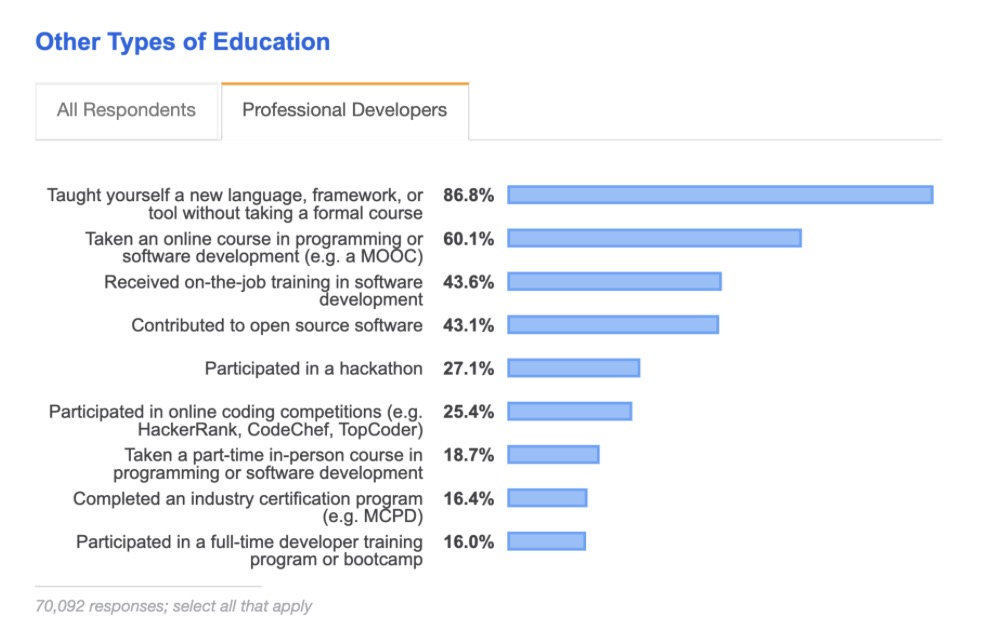
\includegraphics[scale=0.4]{市场分析.png}
\end{center}

而在这些众多的“网课爱好者”编程人员之外,我们平台还聚焦于挖掘潜在的小众用户。这些用户往往有着自己独特的需求,他们可能是刚刚进入工作领域的开发者,也有可能是在某个领域已经有了一定的开发经验,想进一步精进技术的开发人员。这些用户不在大部分的网课受众范围中,往往需要相关领域的专家来开设特定的精品课程才能满足这类人的需求。因此我们平台也设想通过提供此类服务来吸引和挖掘更多的潜在客户。

\subsubsection{需求和诉求}
主要问题:列举市场需求并分析这些需求被满足的程度。

在我们设计的商业模式中可具体化为如下问题:用户对网课的需求是否被满足了?还有潜在的需求没被满足或者等待挖掘吗?

我们调研的结论是:目前的众多网络教育平台不能很好的满足多样的用户需求,例如根据报告\href{https://www.jianshu.com/p/36f272b9895a}{慕课的优缺点},可以看到,慕课“没有分类、分层的教学目标分析”,也没能很好的契合小众用户对专业知识的多样化需求。而这在很多目前的网课平台普遍存在。众多的网络平台依托于大学开设课程,而这些课程往往是“大部头”,需要有长时间的学习以及一定的知识基础。对于一些专业背景知识不足,或是时间不够的用户来说,难以跟进。更重要的是,这些通识课程往往难以满足用户对于专业知识和领域知识的需求。因此我们平台针对用户推出的个性化精品课程有着强大的竞争力。

\subsubsection{切换和成本}
主要问题:客户一旦转投竞争对手,哪些方面需要改变。

在我们设计的商业模式中可具体化为如下问题:用户是否容易脱离我们的平台,转向使用其他的网课平台或是问答平台?

就我们平台而言,我们认为我们平台的用户粘性较高。理由是首先我们有针对小众用户开设的精品课程(见上文讨论),对于这些小众课程的受众来说,我们平台提供了丰富的资源,这些资源在其他网站上很难获得。而且即使其他网站也开设了同样的课程,因为网课内容的高度重合,他们能吸引到的新客户数量也是有限的,考虑到这类小众用户数量本来就少,因此其他平台开设类似课程对他们而言风险也很大。

其次,我们的问答平台和师资团队的优质性让我们可以吸引来大量的提问者和编程学员,而大量的提问者又可以吸引来更多的回答者和老师。因此平台本身会形成良性循环。

最后,由于我们平台集网课和问答于一体,这两部分内容可以相辅相成,对于问答频繁的领域,我们可以开设课程,而对于课程的相关内容,也可以在问答区形成延伸。这种独特的氛围是其他的平台所没有的。


\subsubsection{收入和吸引力}
主要问题:识别与收入心引力和定价能力相关的因素。

在我们设计的商业模式中可具体化为如下问题:平台如何获取收益?如何将问答资源转为平台收入?是否可以从网课中获取收入?

首先我们平台可以从网课中获得提成。通过抽取少量提成,既促进了优秀的老师来开设课程,又可以让平台有一定的收入。其次我们也提供有付费问答的服务,对于一些生僻的问题,只有请行业专家才能解决,为此我们平台专门提供了一对一专属私人服务,这种付费问答定价较高,也是平台的收入之一。问答平台的核心知识资源就是问答本身,这类资源可以吸引来很多流量,而流量本身也可以变现。例如我们可以投放一些广告,或是为我们平台自身的网课来投放广告,这也可以提升我们的收入。

\subsection{行业影响力}
\subsubsection{竞争对手}
主要问题:发现当前的竞争对手和它们的相对优势

我们所提出的商业模式所涉及的领域不少,在不同方面所遇到的有stackoverflow平台,Coursera,中国大学Mooc等平台。

1. StackOverflow,属于IT问答平台的领军平台。其优势在于有高浏览量,在代码问答平台方面有很高的知名度,公认答案质量较高。其劣势在于游客到用户转换率不高,存在多种用户权限,不够自由;问问题得到满意回答的成功率不高,所\href{https://hackernoon.com/the-decline-of-stack-overflow-7cb69faa575d the decline of Stack Overflow}{维护的社区风气存在问题},赚取利润率不高。目标客户细分群体主要是有一定常识的编程开发者,新学习编程的用户存在使用门槛。成本结构:人员成本,包括了开发人员、系统管理人员、设计人员、管理人员、市场人员、销售人员;实物成本,有包括工作场所,租赁的服务器等物理资源;还有前期开发成本,维护成本(\href{https://stackoverflow.blog/2016/11/15/how-we-make-money-at-stack-overflow-2016-edition/}{stackoverflow报告})

2. 中国大学Mooc平台是我们的产品在在线教育方面的竞争对手,其上有非常多与大学或者就业相关的课程,是很多大学生mooc学习的首选平台。其优势在于已经与非常多的大学建立合作关系,甚至有的大学的网课教学也依靠这个平台,因而课程资源非常之多,并且基于免费和平等的价值观念,用户享受这些资源的平均成本很低,有大量的用户群体。而劣势是,课程中老师和学生缺乏交互,考核标准单一,只有课后习题与期末考试,在其上放置课程的难度也需要考量。面向客户细分群体:希望以大学的方式学习大学知识的人。成本结构:人员成本,运营人员,客服,聘请老师费用;前期开发费用,开发或者租赁课程辅助工具的成本,服务器租赁的成本等。(\href{https://x.cnki.net/KCMS/detail/detail.aspx?dbcode=CMFD&dbname=CMFD201601&filename=1015804120.nh&uid=WEEvREcwSlJHSldTTEYzVnBFak5MTnFramlsMnh5RjR5NUZpQzA1a0FZVT0=$9A4hF_YAuvQ5obgVAqNKPCYcEjKensW4ggI8Fm4gTkoUKaID8j8gFw!!&v=MjA1OTk4ZVgxTHV4WVM3RGgxVDNxVHJXTTFGckNVUjdxZlkrUnFGeWpsVmJ6SlZGMjZHN3U0R3RET3I1RWJQSVI=}{Mooc商业模式调研报告})

\subsubsection{行业新进入者}
主要问题:发现新的、崛起的行业对手,判断它们是否利用不同于你的商业模式与你竞争

在在线教育行业方面来说,极客学院是一个新增的竞争对手,与中国大学mooc相对,是面向IT职业教育的在线教育平台(\href{https://baijiahao.baidu.com/s?id=1568297331067975&wfr=spider&for=pc }{IT界蓝翔:极客学院值2200万美元?}),赶在互联网飞速发展的时期,商业化气息更重一点,盈利方式也是通过售卖课程(\href{http://www.quankr.com/gnzx/2019175019.html}{用收费建立互联网教育的真正门槛}),为企业提供职业培训服务等。其优势是,对编程方面课程的针对性极强,课程资源覆盖面广,对其面向的客户细分群体有非常大的吸引力;劣势,推行课程贩售模式,在推广和发展用户阶段可能不那么顺利,需要教育市场,等市场养成习惯。市场准入壁垒:在已经有很多mooc类型在线教育平台流行后,进入市场分一杯羹比较困难。面向客群细分群体:希望进行IT职业教育以扩充知识储备或用于求职的人。成本结构:聘请老师,平台的开发和维护成本,公司实体资源。对我们的商业模式的影响:可能会抢走我们一部分课程学习客户,进而收入来源和利润率产生一定负面影响,但因为我们的课程更有交互性,加上平台继承了问答外卖和文档平台等功能,负面影响有限。

\subsubsection{替代性产品与服务}
主要问题:描述你公司的产品和服务的潜在替代品——包括其他市场和行业的产品和服务

在不同领域有stackoveflow等问答平台,codeshare等实时远程代码共享平台,以及一些mooc平台都可以部分代替我们的服务,但我们公司所提供的docker配置环境,一对一问答,课程学习的结合服务,目前市面上还没有。分别与我们的服务相比,就问答上来说,普通的代码问答没有区别(除了我们提供了docker容器以省去环境对齐的成本),但如果遇上紧急情况,多半不能得到及时响应。实时远程代码共享平台能用于点对点解决bug,但首先需要联系解答人,而我们的平台能帮助减少沟通成本与搜索成本。mooc等教育平台上可以学习课程,但缺乏交互的原因,效率不高(\href{http://media.people.com.cn/n1/2016/0309/c402792-28184701.html}{"MOOC"困境}),我们的平台因为更有交互性,效率会更高。就客户转移上,如果使用了我们的服务,再转向其他替代品后,会或多或少存在一些额外,因而客户产生转移的趋势不大。而这些替代品基本都来自于免费商业模式。

\subsubsection{供应商和其他价值链参与者}
主要问题:在你公司所在的市场中,描述出目前关键的价值链参与者,并发现新崛起的参与者。

价值链上的参与者有:云服务器提供商,合作开发内容的企业与高校,以及平台所依赖技术的相关公司或社区,如docker工具开发社区等。价值链上的参与者都很关键,也都是我们平台所依存的。没有云服务器提供商,自行搭建和维护服务器所产生的成本会远超租赁云服务器的成本;缺乏合作的企业和高校,会使课程资源变得匮乏,无法吸引和留住用户;容器技术的提升与突破,与平台基于容器的业务所产生的成本密切相关,甚至可能会改变平台的服务和价值主张。在参与者上,新崛起的可能有\href{https://www.infoq.cn/article/czBQl3J9QpTfDjJ6Lq6d}{容器技术相关企业}(比如文中的Mirantis)和云服务器相关企业(比如QingCloud)。在收益上,云服务器厂商获得的收益是稳定的,并且会随着平台规模的扩大而增加;企业与高校参与进我们平台的运行后,会获得收入分成收益,这部分参与者与我们平台的联系最紧密,当平台收益大的时候它们收益也是最大的。

\subsubsection{利益相关者}
主要问题:确认哪些参与者可能会影响你的公司和商业模式

当平台获得投资之后,毫无疑问投资者的意向或者要求会显著地影响我们的公司和商业模式,也许要求增加利润率,使平台的服务或者价值主张发生转变,增加价格之类。另外一方面,合作方(企业,高校或者教师)也会影响我们的公司和商业模式,如果有较多的教师对当前的课程模式不满意,公司会考虑改革模式,塑造更良好的教师和学员体验。

当容器技术领域产生变化时,可能会对我们的代码沙盒运行方式,比如使公司应用新产生的技术改善代码沙盒(\href{https://m.sohu.com/n/458230899/}{从容器之热看新时代的虚拟化技术})

\subsection{关键趋势}
\subsubsection{技术趋势}
主要问题:识别威胁到你的商业模式的技术趋势,以及能推动你的商业模式进步的技术趋势

在我们设计的商业模式中可具体化为如下问题:我们的平台利用到了哪些最新的技术,相较于其他平台在技术上有什么优势?

随着通信技术的发展与基础设施的不断完善,\href{https://trends.google.com/trends/explore?date=all&q=docker}{容器技术突飞猛进},本平台会利用这一机遇。根据 \href{https://meta.stackexchange.com/questions/tagged/question-quality}{stackoverflow 的一些统计},许多初学者常常无法确定自己代码的问题所在,没有给出关键信息,从而造成回答者难以回答,增加了沟通成本。相较于传统的问答平台,我们的平台拥有独特的“问答社区”,为每一位问答者提供代码沙箱,简化提问、回答的步骤,提高问答效率。

\subsubsection{行业管理趋势}
主要问题:描述影响你的商业模式的管理规定和管理趋势

在我们设计的商业模式中可具体化为如下问题:国家的那些管理政策或限制会影响到本平台呢?

原本的在线教育行业并没有统一的监管体系,运营较为混乱。2020 年新冠疫情爆发后,全国学校纷纷开始网上教学,国家也立刻出台了\href{http://news.sciencenet.cn/htmlnews/2020/4/438879.shtm}{一系列的管理措施},全国人大教科文卫委也提出要\href{http://www.legaldaily.com.cn/index/content/2020-04/07/content_8163684.htm}{加大网络在线教育监管力度},此举可能会对一些非正规的平台造成一定的影响。我们的平台主要会通过与企业、高校的合作来保证课程质量,严格遵守国家有关规定。

\subsubsection{行业管理趋势}
主要问题:识别可能影响你的商业模式的社会趋势

在我们设计的商业模式中可具体化为如下问题:社会对于编程学习的态度是怎样的?

近年来,软件行业以其高薪而吸引了不少学习者,尤其是青少年,据统计,7-12 岁的青少年群体中,超过 20\% 的人\href{http://scitech.people.com.cn/n1/2020/0327/c1007-31650917.html}{在编程上投入的时间超过语文、数学、英语等 K12 学科},并且 2017 年,国务院印发《新一代人工智能发展规划》明确指出在中小学阶段设置人工智能课程,大力推行\href{https://www.admin5.com/article/20200410/949348.shtml}{编程教育},整个社会对于编程学习趋之若鹜,颇有当年奥数的风范。

\subsubsection{社会经济趋势}
主要问题:总结和你的商业模式有关的主要社会经济趋势

在我们设计的商业模式中可具体化为如下问题:目前大家是否会选择花钱学习编程呢?

答案是肯定的,如上条所述,编程正在成为青少年的“必修课”之一。\href{http://www.xinhuanet.com/2019-11/06/c_1125198958.htm}{根据统计},一名 7 岁儿童每年学习编程需要花费 5000 到 20,000 元,我国少儿编程 2019 年的市场规模大约有 50 亿元,未来两三年内预计还将有3到4倍增长。根据调查结果,2020 年互联网行业春招 Offer 年薪甚至可以拿到 30-40w,\href{https://baijiahao.baidu.com/s?id=1664842639923951399&wfr=spider&for=pc}{远远超过其他行业},巨大的利益使得人们更加愿意在编程学习上投入金钱。

\subsection{宏观经济影响}
\subsubsection{全球市场情况}
主要问题:识别当前经济是否处于爆发期,分析总体市场的情绪,GDP的增长率和失业率等问题

在我们设计的商业模式中可具体化为如下问题:当代的大学生或者资深编程爱好者是否存在大量待业的情况?当前市场中是否存在一些高质量程序员供过于求导致失业率升高的情况?

就目前看来虽然互联网行业整体的发展蒸蒸日上,但是互联网行业大多需要的是新鲜血液,年纪较大的程序员有时会面临失业的情况。通过新闻\href{https://baijiahao.baidu.com/s?id=1650890199865475535&wfr=spider&for=pc}{”腾讯程序员失业3个月,送外卖谋生:人到中年,活成职场“狗不理“}可以看出程序员过了吃“青春饭”的时间之后,往往需要令谋出路,会有大量程序员无法找到合适的工作从而失业。

再加上进来疫情的影响,无论是国内还是国外的GDP都遭受重创,\href{https://3g.163.com/war/article_cambrian/FAKJHGDM0515DN7K.html}{“中国1季度GDP猛降6.8\%,释放5大强烈信号”},\href{http://news.ifeng.com/c/7vvZCnm9p9K}{“一颗“定时炸弹”引爆疫情,新加坡GDP创十年来新低”},\href{https://baijiahao.baidu.com/s?id=1664737589784546565&wfr=spider&for=pc}{“疫情致韩国一季度GDP环比负增长”}这些新闻表明目前全球的经济形势并不景气,这导致许多知名企业进行了大规模裁员,大学生难找到工作也面临失业。根据新闻“年近30,半失业状态:定制化,正在拖垮程序员”https://3g.163.com/all/article/F4UKRGOE0531BCXQ.html可以看出经济寒冬与裁员潮,将是未来常态。

而我们的平台可以为这些程序员提供了就业机会,可以入驻平台成为“解答小哥”,或者开设网课,通过这些方式,缓解大龄程序员的就业问题。

\subsubsection{资本市场}
主要问题:所处的资本市场处于什么状态,获得投资的难易程度以及便捷程度,获取投资的成本有多高。

在我们设计的商业模式中可具体化为如下问题:我们的平台能否顺利获得启动资金进行开发。

现如今教育平台还是比较受欢迎的投资领域,尤其是和互联网相关的教育行业。从新闻\href{https://baijiahao.baidu.com/s?id=1664547183775159480&wfr=spider&for=pc}{“快手3000万美元投资儿童教育启蒙平台火花思维”},\href{https://36kr.com/p/5310719}{“Reliance 向 AI 教育平台 Embibe 追加6600万美元投资。”}看出一些互联网大公司还是非常愿意投资教育平台的。在疫情期间线上教育平台发展迅速,而且还有很大的上升空间。

\subsubsection{大宗商品和其他资源}
主要问题:描述业务必备的大宗商品和其他资源的市场状态,是否容易获取,成本如何?

在我们设计的商业模式中可具体化为如下问题:我们的平台是否容易获取实物资源,知识性资源以及人力资源,以及为了获取这些资源的成本如何?

如今涌现出许许多多的服务器厂商,除了联想,戴尔,华为等主力军之外越来越多的厂商也渐渐出现。通过\href{http://ent.ifeng.com/c/7vsCxpv6us5}{“中国服务器市场添生力军 宁畅布局精细定制领域”}这则新闻发现,现在市场上服务器资源比较充足,容易获得。而且现在已经有了许多课程平台,提问平台,比如MOOC,CSDN等从侧面体现出现在的学习资源也非常丰富。至于开发和维护的人力资源,如今计算机专业大热,有大量程序员涌入市场。


\subsubsection{经济基础设施}
主要问题:如何评价当前市场的基础设施和人民的生活质量?

在我们设计的商业模式中可具体化为如下问题:根据当前人民的生活水准,人们是否有使用CodeOcean平台的经济基础?毋庸置疑,现在人们的生活质量相较于之前已经有了大幅提升,人们的生活需求已经从吃饱穿暖转向提升自己的知识水平上。而且人们想要挣更多的钱,大部分人已经将目光投向互联网行业,开始学习编程,因为这个行业非常有前景。所以当前的经济基础能够支持大部分人学习编程。

\section{评估商业模式}
\subsection{总体评估}

分析:
\begin{center}
  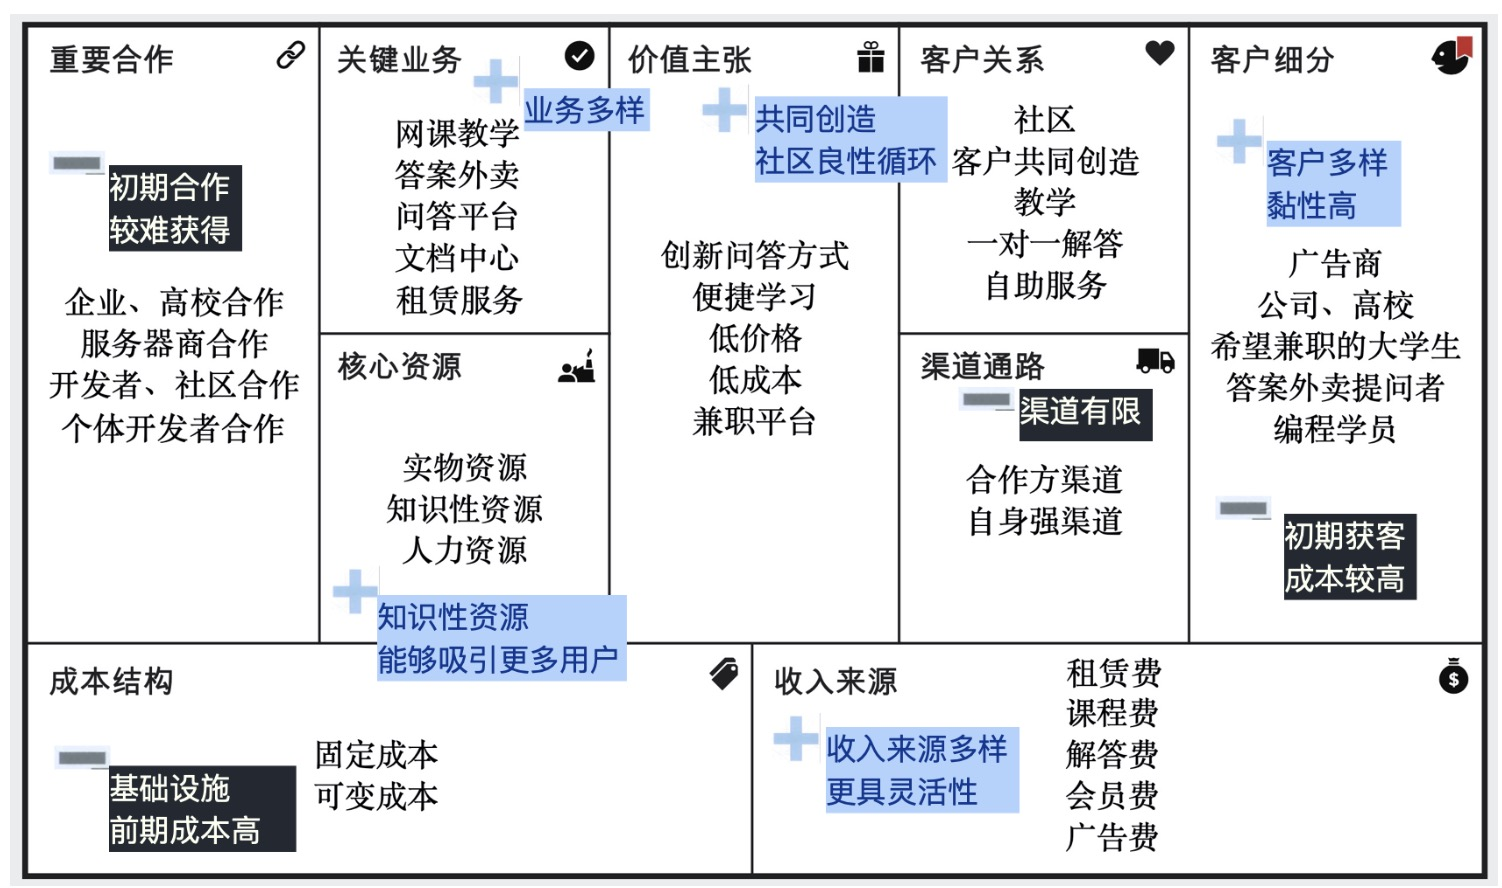
\includegraphics[scale=0.3]{总体评估.png}
\end{center}
我们设计的商业模式总体上是一个网课和问答平台,因此从重要合作和客户的角度上来看,我们的依赖较高。对于平台初期来说,我们面临一定的启动风险,即如何才能吸引来大量的问答用户和课程老师。因为往往一个优秀的回答者在其他网站已经积累了大量的回答记录,在别的平台已经建立起了一整套完整的用户信息和用户生态,对于这类资深回答的用户来说,切换平台的难度较大。因此我们平台在这一块必须要有能够吸引来回答者的优势,例如从付费问答角度考虑。另外,对于其他平台来说,这一类资深用户也是其宝贵资源,因此一定也会采取相应的措施来防止用户的流失。而对于开设课程的老师和工程师来说,吸引他们前来开课相对会简单一些,因为我们平台可以给他们更加灵活的选择,不会占用他们大量的工作时间,也能让他们获得一定的收入,而对于高校老师而言,一份收入不菲的兼职还是具有\href{https://new.qq.com/omn/20190613/20190613A06C5P.html}{一定的吸引力}的。因此目前权衡难易,应该可以从老师和工程师入手,先开设优质的精品课程,然后吸引来学员,进而吸引来提问者和回答者。对于初期阶段来说,我们不可能在规模上取得优势,因此要尽可能在内容上取得优势,而有时\href{https://www.tmtpost.com/42868.html}{内容更甚于规模}。

在我们设计的商业模式中,要求形成用户共同创造的社区氛围,这会在回答者和提问者中形成良性循环。另一方面,客户关系中的一对一解答也是我们平台的特色,主要对应到核心业务中的付费问答,也是收入来源之一,更重要的是,这也是吸引来优质合作者的手段之一。而吸引用户的手段主要还是通过各式各样的广告,或是凭借用户圈子中的口口相传,虽然说\href{https://wiki.mbalib.com/wiki/%E7%86%9F%E4%BA%BA%E7%BB%8F%E6%B5%8E}{熟人的宣传相比传统的宣传手段效果较好},但是在宣传手段上仍然略显单一,这方面可能还有欠缺。

在核心资源方面,为了节约成本,我们平台拟采用docker配合云来实现部署和运维,这将大大降低前期的开发成本,加速平台的发展。此外,后期我们也打算部署我们自己的云服务,因为我们的问答是基于docker的,而目前的其他问答平台基本都无法运行代码,我们可以为他们提供基于docker的问答环境,为每一个问答提供一个docker的租赁服务。目前的市场环境也充分证明了\href{https://www.jianshu.com/p/553b35e0fc82}{docker适合初创公司}。

平台在收入来源上形式还是较为多样的,除了前面提及的付费问答,还涉及用户的部分网课的费用,这部分收入从老师的网课收益中提成,可以根据上课人数动态调整来激发开课教师和工程师的积极性。对应上文提到的核心资源,我们提供的租赁服务也可以提供一定的收入,收入来源的丰富极大的提升了我们平台的灵活性和发展的可能性。

展望:
\begin{center}
  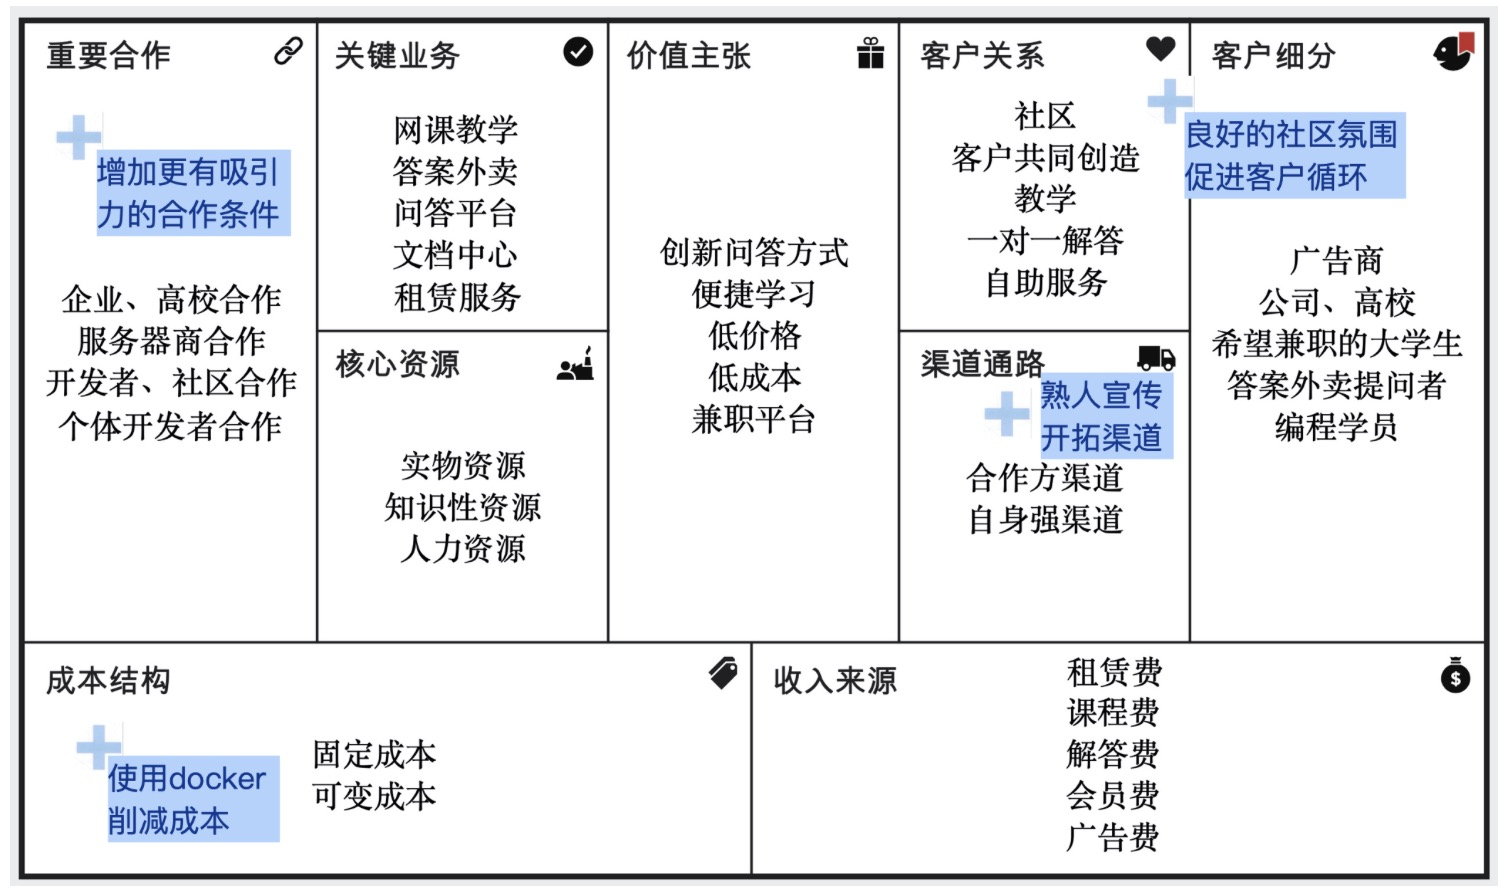
\includegraphics[scale=0.3]{展望.png}
\end{center}
在重要合作方面,主要是针对平台初期的用户,我们需要加大投资的力度,争取通过更有竞争力的薪资合作或是独特的创新思路来吸引优质的师资和工程师;在关键业务方面,加大对于云计算和存储的部署研发,能提供简单的API来使得为每个问题提供一个单独的docker运行环境尽量便捷和轻量级,后续可以提供租赁服务;在核心资源方面,保护我们的问答知识资源;在收入方面,采用多个收入渠道,提升收入的多样性,前期可以做适当的调整,提供一定的免费服务,例如可以减少网课的提成,来吸引更多的老师开设课程,形成一定规模之后再收取部分提成,这样有利于初期吸引更多的用户;在客户关系方面,坚持客户共同创造的社区氛围,形成提问者和回答者之间的互动和良性循环。

\subsection{SWOT}

\begin{table}[h]
  \centering
\begin{tabular}{|p{3.5cm}|c|p{10cm}|}
  \hline
  我们的价值主张良好匹配了客户的需求 & 4 & 我们的创新问答方式、便捷学习和低价格的价值主张满足了答案外卖的提问者和编程学员的需求。兼职平台满足了想要兼职的大学生的需求。\\
  \hline
  我们的价值主张有很强烈的网络效应  & 2 & 在问答平台中,我们平台的价值与提问者和回答者的数量成正比。用户在利用平台的同时,为平台创造资源,创造价值。\\
  \hline
  我们的产品和服务是强耦合的 & 5 & 我们的提供的产品紧紧依赖于我们拥有的服务。我们拥有许许多多网课服务,所以我们为客户提供了线上网课教学的产品;我们拥有 docker 云平台的服务,对应我们为用户提供答案外卖、问答平台等产品。\\
  \hline
  我们的客户很满意 & 5 & 我们平台提供的业务符合用户需求,而且服务水平良好,能够获得客户的好评。\\
  \hline
  我们有很高的利润 & 4 & 我们通过收取课程费、解答费、会员费和广告费来获得利润。\\
  \hline
  我们的收入是可以预期的 & 3 & 我们的收入结构是相对固定的,但是用户使用平台的频率不好预测,可能会在课程费,解答费,会员费上的收入有波动。另外,合作的广告商也不是一成不变的,广告费也可能会有变化。\\
  \hline
  我们有很多经常性收入,有很多回头客 & 4 & 我们的平台特有的业务可以留住顾客,能让用户继续使用我们的平台,继续在平台上消费,使得平台有经常性收入。\\
  \hline
  我们的收益来源是多样化的 & 5 & 我们主要的收入来源来自于:课程费、解答费、会员费、广告费\\
  \hline
  我们的收益来源是可持续的 & 4 & 我们的课程费和会员费可以设置成自动续费的功能,能让用户一直使用我们的平台。\\
  \hline
  我们在支出成本之前就有收入进账 & -5 & 我们在花费成本购入必要资源之前(即平台服务还没有搭建好)还没有收入来源\\
  \hline
  客户真正想买的就是我们提供的 & 5 & 我们深入了解了不同用户的诉求,站在他们的角度思考真正想要什么。比如:提问者想要拥有一个集“代码展示、在线IDE、配置环境的一致性描述、bug可复现、直观呈现修改前后对比”为一体的平台以及拥有一个随叫随到为自己解答问题的人。我们提供的“答案外卖”满足了客户想要。\\
  \hline
  我们的定价机制能够抓住客户全部的购买意愿 & 3 & 我们的课程费和VIP费相对于同类型的平台价格较低,能让用户在对比多家平台之后因为价格低选择我们。\\
  \hline
  我们的成本可以预测 & 5 & 我们的成本结构是固定的,有开发维护的人力成本,服务器的购买成本,以及各种合作费用,宣传费用等。\\
  \hline
  我们的成本结构正确地匹配了我们的商业模式 & 4 & 我们花费一定成本聘请公司、高校教师。这些教师在平台开设课程,供其他用户学习。将不同的用户联系在一起,匹配我们的多边平台商业模式。\\
  \hline
  我们运营的成本效率极高 & 5 & 我们需要定期维护平台和服务器,需要运营费用。\\
  \hline
\end{tabular}
\end{table}

\begin{table}[h]
  \centering
\begin{tabular}{|p{3.5cm}|c|p{10cm}|}
  \hline
  我们从规模经济中获益 & 5 & 当我们扩大平台的规模即增加更多的服务器,这样能够承载更多的用户,有更多的用户使用平台,进行消费。这是我们的平台就会获得更多收益。\\
  \hline
  竞争对手很难复制我们的核心资源 & 4 & 我们的知识性资源很多是用户共同创造的(用户提问,用户解答),竞争对手无法复制。\\
  \hline
  资源的需求可以预测 & 5 & 我们可以根据用户使用平台的流畅程度来预测是否需要更多的服务器资源,平台开发维护的人力资源。\\
  \hline
  我们在正确的时间部署了合适的资源 & 5 & 编程学习逐渐成为社会风气,有学习编程需求的人越来越多,所以我们处在一个正确的时间部署资源。\\
  \hline
  我们有效地执行了关键业务 & 4 & 我们的平台的功能和关键业务一一对应。\\
  \hline
  我们的关键业务很难被复制 & 1 & 我们的“答案外卖”业务在竞品平台中比较少见,比较难被复制,但是“网课教学”、“问答平台”、“文档中心”等业务在众多平台中都有普及,容易被复制。\\
  \hline
  执行质量很高 & 4 & 我们的每一个关键业务都有高质量的执行。\\
  \hline
  我们的自有活动和外包活动达到了理想的平衡 & 5 & 我们的关键业务之间彼此相连,一系列功能都是在编程学习中不可或缺的,用户一般都通过整套流程来提升自己的代码水平。\\
  \hline
  我们很聚焦,并且在必要的时候与伙伴合作 & 5 & 我们聚焦于编程教学,所以非常必要和企业、高校合作\\
  \hline
  我们与重要合作伙伴的关系很融洽 & 5 & 企业、高校是我们的课程来源,我们必须维持良好的合作关系。\\
  \hline
  客户流失率很低 & 5 & 课程的学习需要有上下文的衔接,良好的服务增加了用户对平台的信任,因此用户不会轻易离开。\\
  \hline
  客户群被很好地分类 & 4 & 我们的客户大致分为:广告商、公司高校、希望兼职的大学生、答案外卖的提问者以及编程学员。\\
  \hline
  我们不断地获得新的客户 & 4 & 学员之间的宣传,与高校的合作都能为平台带来新客户。\\
  \hline
  我们的渠道很有效率 & 4 & 我们通过合作方渠道宣传,比如学校企业内开展讲座活动进行宣传能够迅速获得新的用户。\\
  \hline
  我们的渠道有很好的效果 & 4 & 我们通过合作方渠道宣传,比如学校企业内开展讲座活动进行宣传能够迅速获得新的用户。\\
  \hline
  渠道链接客户的能力很强 & 3 & 在合作方渠道中,学校和企业中的关系网密切,容易将潜在的用户链接起来。\\
  \hline
  客户能够轻易地看到我们的渠道 & 2 & 在自身强渠道中,平台是通过服务质量的口碑来提升知名度,用户不容易看到。\\
  \hline
  渠道被高度整合 & 5 & 自身渠道为平台构建基础环境,合作渠道为我们提供初始资源。\\
  \hline
  渠道产生了规模经济 & 5 & 在扩展渠道通路的同时(在更多的企业学校内宣传),可以获得更多用户,从而受益更大。\\
  \hline
\end{tabular}
\end{table}

\begin{table}[h]
  \centering
\begin{tabular}{|p{3.5cm}|c|p{10cm}|}
  \hline
  渠道良好地匹配了客户群体 & 5 & 合作方渠道匹配了企业高效和编程学院等客户群体,自身强渠道匹配了提问者和兼职大学生等客户群体。\\
  \hline
  客户关系强 & 5 & 我们的客户之间联系紧密,比如社区维护了用户之间的关系。\\
  \hline
  关系质量正确地匹配了客户群体 & 4 & 在我们的“答案外卖”业务中的追问功能,确保用户得到满意的解答,提高用户和平台之间的关系质量。\\
  \hline
  客户切换的成本很高,客户和我们绑定了关系 & 5 & 课程的学习需要有上下文的衔接,创立的社区维护了用户关系,因此用户不会轻易离开。\\
  \hline
  我们的品牌很强 & 未知 & 如果我们能源源不断的扩展新用户,一定能打造更强的品牌。\\
  \hline
\end{tabular}
\end{table}

% 我们的价值主张良好匹配了客户的需求 4:我们的创新问答方式、便捷学习和低价格的价值主张满足了答案外卖的提问者和编程学员的需求。兼职平台满足了想要兼职的大学生的需求。

% 我们的价值主张有很强烈的网络效应 2:在问答平台中,我们平台的价值与提问者和回答者的数量成正比。用户在利用平台的同时,为平台创造资源,创造价值。

% 我们的产品和服务是强耦合的 5:我们的提供的产品紧紧依赖于我们拥有的服务。我们拥有许许多多网课服务,所以我们为客户提供了线上网课教学的产品;我们拥有 docker 云平台的服务,对应我们为用户提供答案外卖、问答平台等产品。

% 我们的客户很满意 5:我们平台提供的业务符合用户需求,而且服务水平良好,能够获得客户的好评。

% 我们有很高的利润 4:我们通过收取课程费、解答费、会员费和广告费来获得利润。

% 我们的收入是可以预期的 3;我们的收入结构是相对固定的,但是用户使用平台的频率不好预测,可能会在课程费,解答费,会员费上的收入有波动。另外,合作的广告商也不是一成不变的,广告费也可能会有变化。

% 我们有很多经常性收入,有很多回头客 4:我们的平台特有的业务可以留住顾客,能让用户继续使用我们的平台,继续在平台上消费,使得平台有经常性收入。

% 我们的收益来源是多样化的 5:我们主要的收入来源来自于:课程费、解答费、会员费、广告费

% 我们的收益来源是可持续的 4:我们的课程费和会员费可以设置成自动续费的功能,能让用户一直使用我们的平台。

% 我们在支出成本之前就有收入进账 -5:我们在花费成本购入必要资源之前(即平台服务还没有搭建好)还没有收入来源

% 客户真正想买的就是我们提供的 5:我们深入了解了不同用户的诉求,站在他们的角度思考真正想要什么。比如:提问者想要拥有一个集“代码展示、在线IDE、配置环境的一致性描述、bug可复现、直观呈现修改前后对比”为一体的平台以及拥有一个随叫随到为自己解答问题的人。我们提供的“答案外卖”满足了客户想要。

% 我们的定价机制能够抓住客户全部的购买意愿 3:我们的课程费和VIP费相对于同类型的平台价格较低,能让用户在对比多家平台之后因为价格低选择我们。

% 我们的成本可以预测 5:我们的成本结构是固定的,有开发维护的人力成本,服务器的购买成本,以及各种合作费用,宣传费用等。

% 我们的成本结构正确地匹配了我们的商业模式 4:我们花费一定成本聘请公司、高校教师。这些教师在平台开设课程,供其他用户学习。将不同的用户联系在一起,匹配我们的多边平台商业模式。
	
% 我们运营的成本效率极高 5:我们需要定期维护平台和服务器,需要运营费用。

% 我们从规模经济中获益 5:当我们扩大平台的规模即增加更多的服务器,这样能够承载更多的用户,有更多的用户使用平台,进行消费。这是我们的平台就会获得更多收益。

% 竞争对手很难复制我们的核心资源 4:我们的知识性资源很多是用户共同创造的(用户提问,用户解答),竞争对手无法复制。

% 资源的需求可以预测 5:我们可以根据用户使用平台的流畅程度来预测是否需要更多的服务器资源,平台开发维护的人力资源。

% 我们在正确的时间部署了合适的资源 5:编程学习逐渐成为社会风气,有学习编程需求的人越来越多,所以我们处在一个正确的时间部署资源。

% 我们有效地执行了关键业务 4:我们的平台的功能和关键业务一一对应。

% 我们的关键业务很难被复制 1:我们的“答案外卖”业务在竞品平台中比较少见,比较难被复制,但是“网课教学”、“问答平台”、“文档中心”等业务在众多平台中都有普及,容易被复制。

% 执行质量很高 4:我们的每一个关键业务都有高质量的执行。

% 我们的自有活动和外包活动达到了理想的平衡 5:我们的关键业务之间彼此相连,一系列功能都是在编程学习中不可或缺的,用户一般都通过整套流程来提升自己的代码水平。

% 我们很聚焦,并且在必要的时候与伙伴合作 5:我们聚焦于编程教学,所以非常必要和企业、高校合作

% 我们与重要合作伙伴的关系很融洽 5:企业、高校是我们的课程来源,我们必须维持良好的合作关系。

% 客户流失率很低 5:课程的学习需要有上下文的衔接,良好的服务增加了用户对平台的信任,因此用户不会轻易离开。

% 客户群被很好地分类 4:我们的客户大致分为:广告商、公司高校、希望兼职的大学生、答案外卖的提问者以及编程学员。

% 我们不断地获得新的客户 4:学员之间的宣传,与高校的合作都能为平台带来新客户。

% 我们的渠道很有效率 4:我们通过合作方渠道宣传,比如学校企业内开展讲座活动进行宣传能够迅速获得新的用户。

% 我们的渠道有很好的效果 4:我们通过合作方渠道宣传,比如学校企业内开展讲座活动进行宣传能够迅速获得新的用户。

% 渠道链接客户的能力很强 3:在合作方渠道中,学校和企业中的关系网密切,容易将潜在的用户链接起来。

% 客户能够轻易地看到我们的渠道 2:在自身强渠道中,平台是通过服务质量的口碑来提升知名度,用户不容易看到。

% 渠道被高度整合 5:自身渠道为平台构建基础环境,合作渠道为我们提供初始资源。

% 渠道产生了规模经济 5:在扩展渠道通路的同时(在更多的企业学校内宣传),可以获得更多用户,从而受益更大。

% 渠道良好地匹配了客户群体 5:合作方渠道匹配了企业高效和编程学院等客户群体,自身强渠道匹配了提问者和兼职大学生等客户群体。

% 客户关系强 5:我们的客户之间联系紧密,比如社区维护了用户之间的关系。

% 关系质量正确地匹配了客户群体 4:在我们的“答案外卖”业务中的追问功能,确保用户得到满意的解答,提高用户和平台之间的关系质量。

% 客户切换的成本很高,客户和我们绑定了关系 5:课程的学习需要有上下文的衔接,创立的社区维护了用户关系,因此用户不会轻易离开。

% 我们的品牌很强 未知:如果我们能源源不断的扩展新用户,一定能打造更强的品牌。

\FloatBarrier
\subsection{机会评估}
\subsubsection{价值主张中的机会}
\begin{table}[h]
  \centering
\begin{tabular}{|p{3.5cm}|c|p{10cm}|}
  \hline
  我们可以将产品转化为服务来获得重复增加的营收吗 & 3 & 可以考虑将我们平台的产品转变为一种服务,向特定客户提供。比如,提供docker出租服务,为企业提供可伸缩的带环境订制和管理服务;为企业搭建企业内部的问答、文档平台,隔离外网环境,建造简单直接的企业内交流社区;对课程教学进行扩展,聘请一些教师/经验工作者,向企业提供员工培训服务。\\
  \hline
  我们能更好地整合我们的产品或者服务吗 & 3 & 可以在不同的服务间建立更强的联系。在问答平台问到一些某门课程相关的知识时,提供链接,引导用户至该门课程;问答平台可以支持附带课程tag信息,让其他同样修习这门课程的学员在浏览问答区的时候更容易看见。\\
  \hline
  我们还可以满足哪些额外的客户需求 & 1 & 客户的需求已经基本满足了,更多的需求比如通过课程学习且有一定编程经验后,希望寻找的求职平台过于庞大,无法集成进当前平台中。\\
  \hline
  还存在与我们的价值主张互补或是延申的东西吗 & 1 & 无。\\
  \hline
  在服务客户的过程中,我们还可以为客户做哪些其他工作 & 2 & 设立与培训客服,获得用户的反馈,帮客户解决问题或者用以改进平台。\\
  \hline
\end{tabular}
\end{table}

% 我们可以将产品转化为服务来获得重复增加的营收吗 3:可以考虑将我们平台的产品转变为一种服务,向特定客户提供。比如,提供docker出租服务,为企业提供可伸缩的带环境订制和管理服务;为企业搭建企业内部的问答、文档平台,隔离外网环境,建造简单直接的企业内交流社区;对课程教学进行扩展,聘请一些教师/经验工作者,向企业提供员工培训服务。

% 我们能更好地整合我们的产品或者服务吗 3:可以在不同的服务间建立更强的联系。在问答平台问到一些某门课程相关的知识时,提供链接,引导用户至该门课程;问答平台可以支持附带课程tag信息,让其他同样修习这门课程的学员在浏览问答区的时候更容易看见。

% 我们还可以满足哪些额外的客户需求 1:客户的需求已经基本满足了,更多的需求比如通过课程学习且有一定编程经验后,希望寻找的求职平台过于庞大,无法集成进当前平台中。

% 还存在与我们的价值主张互补或是延申的东西吗 1:无

% 在服务客户的过程中,我们还可以为客户做哪些其他工作?2:设立与培训客服,获得用户的反馈,帮客户解决问题或者用以改进平台。

\FloatBarrier
\subsubsection{成本收入中的机会}
\begin{table}[h]
  \centering
\begin{tabular}{|p{3.5cm}|c|p{10cm}|}
  \hline
  我们可以将一次性交易收入转换成经常性收入吗 & 2 & 已经设立了会员制度,可以将一次性的课程费用转换为长时期的时间租赁费用;会员自动续费可以增加收入。\\
  \hline
  还有什么产品或服务是客户愿意付费的吗 & 5 & 可以为一些课程建立合集,作为套餐打包出售,作为新的产品;可以面向企业提供搭建和维护内部问答平台的服务,帮助其员工建立一个可以讨论和记录问题的空间。\\
  \hline
  在我们内或者合作伙伴那有没有交叉销售的机会 & 3 & 可以与合作企业,服务器厂商建立交叉合作关系,服务器厂商增加了服务器租赁订单,获得员工培训服务或者其他服务优惠,降低了服务器价格;合作企业获得服务器租赁优惠,获得员工培训服务或者其他服务优惠,帮助我们公司建设课程;我们的公司获得服务器租赁优惠和企业课程建设助理,为合作伙伴提供优惠服务。\\
  \hline
  我们还能增加或创造出其他的收入来源吗 & 1 & 请参考条目2。\\
  \hline
  我们能否提高价格 & 4 & 当用户基数提升后,可以将课程分级以适配多层的用户人群,更高级的课程内容更好,价格更高,通过向目标人群更精准地投放提升课程收入。\\
  \hline
  我们在哪个环节可以缩减成本 & 1 & 无,已经通过云服务商削减了服务器的成本。\\
  \hline
\end{tabular}
\end{table}

% 我们可以将一次性交易收入转换成经常性收入吗 2:已经设立了会员制度,可以将一次性的课程费用转换为长时期的时间租赁费用;会员自动续费可以增加收入

% 还有什么产品或服务是客户愿意付费的吗 5:可以为一些课程建立合集,作为套餐打包出售,作为新的产品;可以面向企业提供搭建和维护内部问答平台的服务,帮助其员工建立一个可以讨论和记录问题的空间。

% 在我们内或者合作伙伴那有没有交叉销售的机会 3:可以与合作企业,服务器厂商建立交叉合作关系,服务器厂商增加了服务器租赁订单,获得员工培训服务或者其他服务优惠,降低了服务器价格;合作企业获得服务器租赁优惠,获得员工培训服务或者其他服务优惠,帮助我们公司建设课程;我们的公司获得服务器租赁优惠和企业课程建设助理,为合作伙伴提供优惠服务。

% 我们还能增加或创造出其他的收入来源吗 1:请参考条目2。

% 我们能否提高价格 4:当用户基数提升后,可以将课程分级以适配多层的用户人群,更高级的课程内容更好,价格更高,通过向目标人群更精准地投放提升课程收入。

% 我们在哪个环节可以缩减成本 1:无,已经通过云服务商削减了服务器的成本。

\FloatBarrier
\subsubsection{基础设施中的机会}

\begin{table}[h]
  \centering
\begin{tabular}{|p{3.5cm}|c|p{10cm}|}
  \hline
  我们能否在保持相同结果的同时,使用成本更低的资源 & 1 & 已经通过租用云服务器的方式大幅降低了原本自己维护服务器所需的成本。\\
  \hline
  哪种核心资源从合作伙伴那获取效果会更好点 & 1 & 服务器资源通过租赁获得,如果能与云服务器厂商建立合作关系(已经考虑到)可以获得更低的价格;课程和人力资源通过与企业与高校的合作关系获得。\\
  \hline
  哪种核心资源没有得到充分利用 & 1 & 都已经得到充分利用:租赁云服务器的方式可以灵活地增减服务器,并且也可以通过出租docker的方式利用闲置的服务器资源;课程资源不会损耗,当平台知名度越大时使用的人数为此付费的人数会越多。\\
  \hline
  我们有没有什么未使用过的有价值的知识产权吗 & 1 & 无,目前文档和课程这类知识性资源已经整合进我们的业务中了。\\
  \hline
  我们可以对某些关键业务实施标准化流程吗 & 1 & 无。\\
  \hline
  我们该如何从整体上提高效率 & 2 & 决定好公司中的部门与职责划分,以及沟通规范,提高公司运行效率。\\
  \hline
  IT技术支持能提高效率吗 & 1 & 平台本身已经建立在IT技术的基础上。\\
  \hline
  是不是存在一些业务外包的可能 & 3 & 如果有条件,平台早期的开发可以外包给专业的互联网公司,公司本身可以专注于容器相关技术的研究与开发。\\
  \hline
  与合作伙伴更深入的合作是否有助于我们更专注核心业务 & 5 & 当与企业和高校的合作关系深入后,课程数量一定会增加,吸引来更多的客户,我们平台可以更致力于社区的建设与维护,减少在寻求更多合作伙伴之上的精力花费\\
  \hline
  在我们与合作伙伴的关系中存在交叉销售的机会吗 & 1 & 无。\\
  \hline
  我们合作伙伴的渠道通路可以帮助我们接触客户吗 & 5 & 合作的企业和高校的宣传可以帮助我们平台提升知名度,由合作企业的推荐可以更简单地与别的企业建立关系,由此与其合作推出课程或者为其提供面向企业的服务。\\
  \hline
  我们的合作伙伴能够补充我们的价值主张吗 & 1 & 无。\\
  \hline
\end{tabular}
\end{table}
% 我们能否在保持相同结果的同时,使用成本更低的资源 1:已经通过租用云服务器的方式大幅降低了原本自己维护服务器所需的成本。

% 哪种核心资源从合作伙伴那获取效果会更好点 1:服务器资源通过租赁获得,如果能与云服务器厂商建立合作关系(已经考虑到)可以获得更低的价格;课程和人力资源通过与企业与高校的合作关系获得。

% 哪种核心资源没有得到充分利用 1:都已经得到充分利用:租赁云服务器的方式可以灵活地增减服务器,并且也可以通过出租docker的方式利用闲置的服务器资源;课程资源不会损耗,当平台知名度越大时使用的人数为此付费的人数会越多。

% 我们有没有什么未使用过的有价值的知识产权吗 1:无,目前文档和课程这类知识性资源已经整合进我们的业务中了。

% 我们可以对某些关键业务实施标准化流程吗 1:无。

% 我们该如何从整体上提高效率 2:决定好公司中的部门与职责划分,以及沟通规范,提高公司运行效率。

% IT技术支持能提高效率吗 1:平台本身已经建立在IT技术的基础上。

% 是不是存在一些业务外包的可能 3:如果有条件,平台早期的开发可以外包给专业的互联网公司,公司本身可以专注于容器相关技术的研究与开发。

% 与合作伙伴更深入的合作是否有助于我们更专注核心业务 5:当与企业和高校的合作关系深入后,课程数量一定会增加,吸引来更多的客户,我们平台可以更致力于社区的建设与维护,减少在寻求更多合作伙伴之上的精力花费

% 在我们与合作伙伴的关系中存在交叉销售的机会吗 1:无。

% 我们合作伙伴的渠道通路可以帮助我们接触客户吗 5:合作的企业和高校的宣传可以帮助我们平台提升知名度,由合作企业的推荐可以更简单地与别的企业建立关系,由此与其合作推出课程或者为其提供面向企业的服务。

% 我们的合作伙伴能够补充我们的价值主张吗 1:无。

\FloatBarrier
\subsubsection{客户界面中的机会}
\begin{table}[h]
  \centering
\begin{tabular}{|p{3.5cm}|c|p{10cm}|}
  \hline
  我们应该怎样利用日益壮大的市场 & 3 & 考虑到我们公司是通过结合已有的商业模式并创造额外价值,因此这片市场的竞争者还很少,可以充分宣传平台,吸引用户,如果在早期在市场所占的份额足够高,可以建立该行业的权威形象,扩大平台,在该行业中立稳脚跟。\\
  \hline
  我们能服务新的客户细分群体吗 & 1 & 在目前的平台框架下,无法再整合出更大的客户总群体。\\
  \hline
  我们恁通过更为精细的客户细分群体来更好地服务客户吗 & 4 & 可以建立更精细的编程学员模型,根据其编程经验进行细分,相对应地为课程分级,对不同经验等级的客户投放不同等级的课程,以更精准地满足其学习需求。\\
  \hline
  我们该如何改善我们渠道通路的效率和效能 & 3 & 推出新方法,鼓励教师线下宣传该平台,能更好地渗透学生用户群体;用课程优惠券或者答案外卖优惠券鼓励用户邀请新用户。\\
  \hline
  我们能更好地整合我们的渠道通路吗 & 1 & 无。\\
  \hline
  我们能在合作伙伴那发现与我们的渠道具有互补性的渠道通路吗 & 1 & 无。\\
  \hline
  我们可以直接服务我们的客户来提高我们的利润率吗 & 3 & 可以开展面向企业的服务,如成本收入机会的条目2,直接服务企业,增加利润。\\
  \hline
  我们能否更好地平衡渠道通路与客户细分群体之间的关系 & 2 & 渠道与客户的关系基本已经确定了,公司与高校是我们公司的重要合作伙伴,前期会把重点放在通过自身渠道来接触到该群体并建立合作关系,待推出足够多的资源,社区建立初具规模后可以将渠道通路重点向希望兼职的大学生或者编程学员方面倾斜,并且鼓励他们邀请更多的人来使用我们平台。\\
  \hline
  在针对客户的售后服务上,还有什么改进的空间吗 & 3 & 目前公司决定在问答区或者课程区都设立客服以解决售后问题;培训客服以更好地解决问题。\\
  \hline
  我们应该如何加强我们与客户之间的关系 & 3 & 我们可以在问答社区中设立多种用户权限,较高级的用户可以类似监督之类帮助维护社区,由此可以让问答社区环境更好,提升整体用户与平台的关系,高权限的用于与平台的关系也会更紧密。\\
  \hline
\end{tabular}
\end{table}

\begin{table}[h]
  \centering
\begin{tabular}{|p{3.5cm}|c|p{10cm}|}
\hline
我们能在服务的个性化上加以改善吗 & 5 & 在用户需要答案外卖解答者时,平台为其筛选/匹配适合其的解答者,降低用户的搜寻成本。\\
\hline
我们应该怎样来提高客户的转移成本 & 5 & 通过改善问答平台课程平台各子平台的服务水平,更紧密地联系这些子平台,提升不可替代性。\\
\hline
我们是否已经发现并放起了不能未我们带来收益的客户,如果没有,为什么 & 1 & 严格来说只有一类不适用答案外卖而只使用问答平台(类似浏览stackoverflow)的用户不会直接为平台带来收益。但这类用户基数较大,客观上有起到帮助宣传平台的作用,并且其也是潜在的付费用户,如果平台推出了其感兴趣的资源,可以将其中一些用户转化为付费用户。\\
\hline
我们需要自主化一些关系吗 & 1 & 不需要。\\
\hline
\end{tabular}
\end{table}
% 我们应该怎样利用日益壮大的市场 3:考虑到我们公司是通过结合已有的商业模式并创造额外价值,因此这片市场的竞争者还很少,可以充分宣传平台,吸引用户,如果在早期在市场所占的份额足够高,可以建立该行业的权威形象,扩大平台,在该行业中立稳脚跟。

% 我们能服务新的客户细分群体吗 1:在目前的平台框架下,无法再整合出更大的客户总群体。

% 我们恁通过更为精细的客户细分群体来更好地服务客户吗 4:可以建立更精细的编程学员模型,根据其编程经验进行细分,相对应地为课程分级,对不同经验等级的客户投放不同等级的课程,以更精准地满足其学习需求。

% 我们该如何改善我们渠道通路的效率和效能 3:推出新方法,鼓励教师线下宣传该平台,能更好地渗透学生用户群体;用课程优惠券或者答案外卖优惠券鼓励用户邀请新用户。

% 我们能更好地整合我们的渠道通路吗 1:无。

% 我们能在合作伙伴那发现与我们的渠道具有互补性的渠道通路吗 1:无。

% 我们可以直接服务我们的客户来提高我们的利润率吗 3:可以开展面向企业的服务,如成本收入机会的条目2,直接服务企业,增加利润。

% 我们能否更好地平衡渠道通路与客户细分群体之间的关系 2:渠道与客户的关系基本已经确定了,公司与高校是我们公司的重要合作伙伴,前期会把重点放在通过自身渠道来接触到该群体并建立合作关系,待推出足够多的资源,社区建立初具规模后可以将渠道通路重点向希望兼职的大学生或者编程学员方面倾斜,并且鼓励他们邀请更多的人来使用我们平台。

% 在针对客户的售后服务上,还有什么改进的空间吗 3:目前公司决定在问答区或者课程区都设立客服以解决售后问题;培训客服以更好地解决问题。

% 我们应该如何加强我们与客户之间的关系 3:我们可以在问答社区中设立多种用户权限,较高级的用户可以类似监督之类帮助维护社区,由此可以让问答社区环境更好,提升整体用户与平台的关系,高权限的用于与平台的关系也会更紧密。

% 我们能在服务的个性化上加以改善吗 5:在用户需要答案外卖解答者时,平台为其筛选/匹配适合其的解答者,降低用户的搜寻成本。

% 我们应该怎样来提高客户的转移成本 5:通过改善问答平台课程平台各子平台的服务水平,更紧密地联系这些子平台,提升不可替代性。

% 我们是否已经发现并放起了不能未我们带来收益的客户,如果没有,为什么 1:严格来说只有一类不适用答案外卖而只使用问答平台(类似浏览stackoverflow)的用户不会直接为平台带来收益。但这类用户基数较大,客观上有起到帮助宣传平台的作用,并且其也是潜在的付费用户,如果平台推出了其感兴趣的资源,可以将其中一些用户转化为付费用户。

% 我们需要自主化一些关系吗 1:不需要。

\FloatBarrier
\subsection{评估威胁}
\subsubsection{对价值主张}
\begin{table}[h]
  \centering
\begin{tabular}{|p{3.5cm}|c|p{10cm}|}
  \hline
  存在可替代的产品和服务吗 & 3 & 我们的部分功能在其他平台上也有体现,比如网课,问答平台,文档中心等。但是目前还没有“答案外卖”相关的平台。\\
  \hline
  竞争对手会报出更有竞争力的价格,或者提供更好的价值吗 & 4 & 有可能他们会搜集到更多的网课资源,文档资源。或者以更低的成本获取这些资源,从而降低用户所需要支付的课程费用,VIP费。\\
  \hline
\end{tabular}
\end{table}
% 存在可替代的产品和服务吗?3:我们的部分功能在其他平台上也有体现,比如网课,问答平台,文档中心等。但是目前还没有“答案外卖”相关的平台。

% 竞争对手会报出更有竞争力的价格,或者提供更好的价值吗?4:有可能他们会搜集到更多的网课资源,文档资源。或者以更低的成本获取这些资源,从而降低用户所需要支付的课程费用,VIP费。

\FloatBarrier
\subsubsection{对成本/收入}
\begin{table}[h]
  \centering
\begin{tabular}{|p{3.5cm}|c|p{10cm}|}
  \hline
  我们的利润受到竞争对手的威胁吗?是技术原因造成的吗? & 3 & 市面上存在一些和我们竞争的产品,可能会因此分流走一部分的客户资源。但技术层面上相差不大。\\
  \hline
  我们过多的依赖某一项或者多项收益来源吗? & 1 & 没有过分依赖。\\
  \hline
  未来哪些收益来源会消失? & 2 & 收益来源大部分和平台功能息息相关。只要平台仍然维持当前的功能,课程费,解答费,会员费不会消失。但如果平台有了自身的强渠道,就不需要广告赞助了。可能广告费会消失。\\
  \hline
  哪几项成本会变得无法预测? & 2 & 当前市场上的实物资源,知识性资源,人力资源的成本比较固定。但是可能由于疫情原因,这些资源的价格可能会有轻微上调。\\
  \hline
  哪些成本的增加会快过他们所支撑的收入?& 2 & 如果平台引进了一些过于小众的网课资源,可能导致观看的用户不多,但是仍然要花费成本获得课程资源。可能会导致课程费用的收入小于购买知识性资源的成本。\\
  \hline
\end{tabular}
\end{table}
% 我们的利润受到竞争对手的威胁吗?是技术原因造成的吗?3:市面上存在一些和我们竞争的产品,可能会因此分流走一部分的客户资源。但技术层面上相差不大。

% 我们过多的依赖某一项或者多项收益来源吗?1:没有过分依赖

% 未来哪些收益来源会消失?2:收益来源大部分和平台功能息息相关。只要平台仍然维持当前的功能,课程费,解答费,会员费不会消失。但如果平台有了自身的强渠道,就不需要广告赞助了。可能广告费会消失。

% 哪几项成本会变得无法预测?2:当前市场上的实物资源,知识性资源,人力资源的成本比较固定。但是可能由于疫情原因,这些资源的价格可能会有轻微上调。

% 哪些成本的增加会快过他们所支撑的收入? 2:如果平台引进了一些过于小众的网课资源,可能导致观看的用户不多,但是仍然要花费成本获得课程资源。可能会导致课程费用的收入小于购买知识性资源的成本。

\FloatBarrier
\subsubsection{对基础设施的威胁}
\begin{table}[h]
  \centering
\begin{tabular}{|p{3.5cm}|c|p{10cm}|}
  \hline
  我们会面临某些资源的供应短缺吗? & 1 & 如今市场上的服务器厂商有很多,而且网课资源丰富,从事编程行业的人很多,所以开发平台的人力资源也很丰富。\\
  \hline
  资源的质量能够保证吗? & 3 & 为了保护资源的质量,我们需要专门设置课程资源的审核分级人员。\\
  \hline
  哪些关键业务会被打扰?& 1 & 不会,如今的外部力量不会打扰到我们的关键业务。\\
  \hline
  我们的活动质量会受到威胁吗?& 3 & 如今用户的水平参差不齐,在问答平台中不一定能保证回答的完全正确。\\
  \hline
  我们有可能会失去哪些合作伙伴?& 1 & 不会\\
  \hline
  我们的合作伙伴有可能和竞争对手合作吗?& 4 & 我们合作的企业和高校可能会在多个平台都发布网课。合作的服务器商也可能为其他平台提供服务器资源。\\
  \hline
  我们是不是过分依赖某些合作伙伴了?& 1 & 我们依赖的合作伙伴是众多的企业,高校,服务器商,开发者和社区,不存在过分依赖某一家的问题。\\
  \hline
\end{tabular}
\end{table}
% 我们会面临某些资源的供应短缺吗?1:如今市场上的服务器厂商有很多,而且网课资源丰富,从事编程行业的人很多,所以开发平台的人力资源也很丰富。

% 资源的质量能够保证吗?3:为了保护资源的质量,我们需要专门设置课程资源的审核分级人员。

% 哪些关键业务会被打扰?1:不会,如今的外部力量不会打扰到我们的关键业务。

% 我们的活动质量会受到威胁吗?3:如今用户的水平参差不齐,在问答平台中不一定能保证回答的完全正确。

% 我们有可能会失去哪些合作伙伴?1:不会

% 我们的合作伙伴有可能和竞争对手合作吗?4:我们合作的企业和高校可能会在多个平台都发布网课。合作的服务器商也可能为其他平台提供服务器资源。

% 我们是不是过分依赖某些合作伙伴了?1:我们依赖的合作伙伴是众多的企业,高校,服务器商,开发者和社区,不存在过分依赖某一家的问题。

\FloatBarrier
\subsubsection{客户界面上的威胁}
\begin{table}[h]
  \centering
\begin{tabular}{|p{3.5cm}|c|p{10cm}|}
  \hline
  我们的市场很快会饱和吗?& 1 & 不会,如今互联网行业的发展迅猛,越来越多的人开始学习编程。\\
  \hline
  有竞争对手在威胁我们的市场份额吗?& 4 & 有。比如MOOC平台的教学资源主要以周期比较长的大课为主,适合一些想要系统性学习的学员。而我们的平台主打短小简介的小课以解决问题为主。\\
  \hline
  客户转投竞争对手的可能性有多高?& 3 & 可能会有一部分客户会尝试MOOC,网易云课堂这样的教学平台。有的倾向于使用CSDN,StackOverFlow这样的问答平台。但是我们平台特有的“答案外卖”可以留住很大一部分用户。\\
  \hline
  我们市场中的竞争多快会变得白热化?& 3 & 我们的平台和竞争对手的平台各自有各自的特点,并不是完全对立的,不会很快竞争白热化。但是又有一部分的功能是相似的,会产生一些用户的竞争。\\
  \hline
  竞争对手会威胁我们的渠道吗?& 2 & 在合作方渠道上,竞争对手可能也会利用高校,企业进行宣传。\\
  \hline
  我们的渠道有变得和客户不相关的危险吗?& 1 & 没有,都是和客户直接接触的,息息相关。\\
  \hline
  我们的客户关系有可能恶化吗?& 3 & 在问答平台和答案外卖中,用户可能会对某些解答不满意,所以要建立良好的售后服务,比如追问追答的功能。\\
  \hline
\end{tabular}
\end{table}
% 我们的市场很快会饱和吗?1:不会,如今互联网行业的发展迅猛,越来越多的人开始学习编程。

% 有竞争对手在威胁我们的市场份额吗?4:有。比如MOOC平台的教学资源主要以周期比较长的大课为主,适合一些想要系统性学习的学员。而我们的平台主打短小简介的小课以解决问题为主。

% 客户转投竞争对手的可能性有多高? 3:可能会有一部分客户会尝试MOOC,网易云课堂这样的教学平台。有的倾向于使用CSDN,StackOverFlow这样的问答平台。但是我们平台特有的“答案外卖”可以留住很大一部分用户。

% 我们市场中的竞争多快会变得白热化? 3:我们的平台和竞争对手的平台各自有各自的特点,并不是完全对立的,不会很快竞争白热化。但是又有一部分的功能是相似的,会产生一些用户的竞争。

% 竞争对手会威胁我们的渠道吗?2:在合作方渠道上,竞争对手可能也会利用高校,企业进行宣传。

% 我们的渠道有变得和客户不相关的危险吗?1:没有,都是和客户直接接触的,息息相关。

% 我们的客户关系有可能恶化吗? 3:在问答平台和答案外卖中,用户可能会对某些解答不满意,所以要建立良好的售后服务,比如追问追答的功能。
\FloatBarrier
\section{蓝海战略}
\subsection{对客户的影响}
\begin{center}
  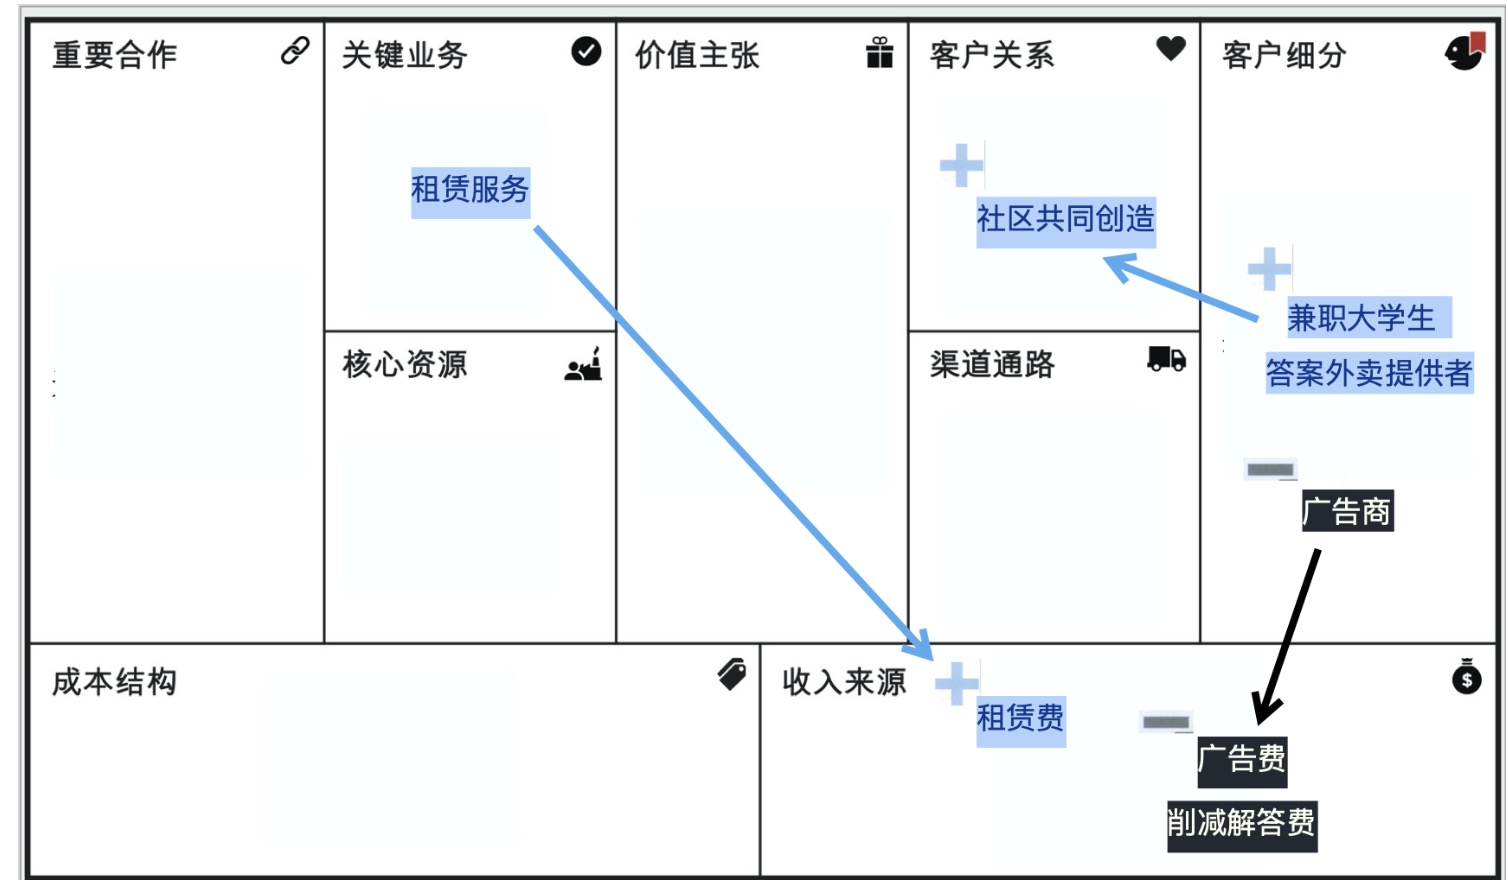
\includegraphics[scale=0.3]{客户影响.png}
\end{center}

\begin{itemize}
  \item \textbf{删除}:广告商
  \item \textbf{削减}:广告费、解答费
  \item \textbf{增加}:兼职大学生、答案外卖提问者
  \item \textbf{创造}:租赁费、社区共同创造的客户关系
\end{itemize}


我们构思的商业模式聚焦于教育,聚焦于为用户解决知识性的问题。正如前文分析,无论是线上教育教育市场,还是问答平台,都存在一定的缺口。因此专注于继续开拓这些市场,挖掘潜在用户是我们平台的主要方向。而对于这类知识性的网站,用户对于广告是很敏感的。如果过多的出现广告,对于用户体验会造成极大的负面影响。

对于广告的内容来说,能够展示的内容也是很有限的。因为首先我们不可能为存在竞争关系的其他网课平台打广告,其次如果删除广告部分,对我们的收入也不会造成实质的影响。权衡利弊,应该要删除广告商这一客户群体。

在收入来源部分,注意到同时存在解答费和会员费。这里应该需要细化一下,例如对已经付费的会员来说,考虑取消其问题的解答费,或是采用一些优惠政策。这样如果用户开通了会员,就可以免费或是以极低的额外成本来使用平台的各项其他服务,减少了收费项目,有利于促进普通用户转向会员的转化率。

减少付费项目的条目的另一个考虑就是促进社区共同创造的客户关系。对于网课和问答平台来说,应该营造一种开源共享和创造的气氛,如果付费项目过多,对这种风气无疑会造成负面影响。

为了平台的长远发展,我们应该从最有发展潜力的客户群体入手。我们平台的特色之一就是解答服务,通过挖掘优秀的大学生来引起一个大的群体的注意,这些大学生不仅是问题的回答者,也是潜在的提问者。大量大学生的加入不仅对于问答平台的问题和答案本身是一个极大的增益,对于社区共同创造的氛围也是起到一个积极影响。

在上文对于基础设施的分析中,我们提到docker化的趋势。我们平台特色的docker问题环境无疑是一个非常具有竞争力的新概念。可以创新地创造出一系列的收入来源,如租赁费和后期的运维收费。这一部分收入来源和我们的主要业务没有直接的关联,主要是通过技术手段来盈利,可以说是一个单独的发展方向。创造这一个收入来源可以大大增加我们平台的灵活性和发展的可能性。

\subsection{价值主张}
\begin{center}
  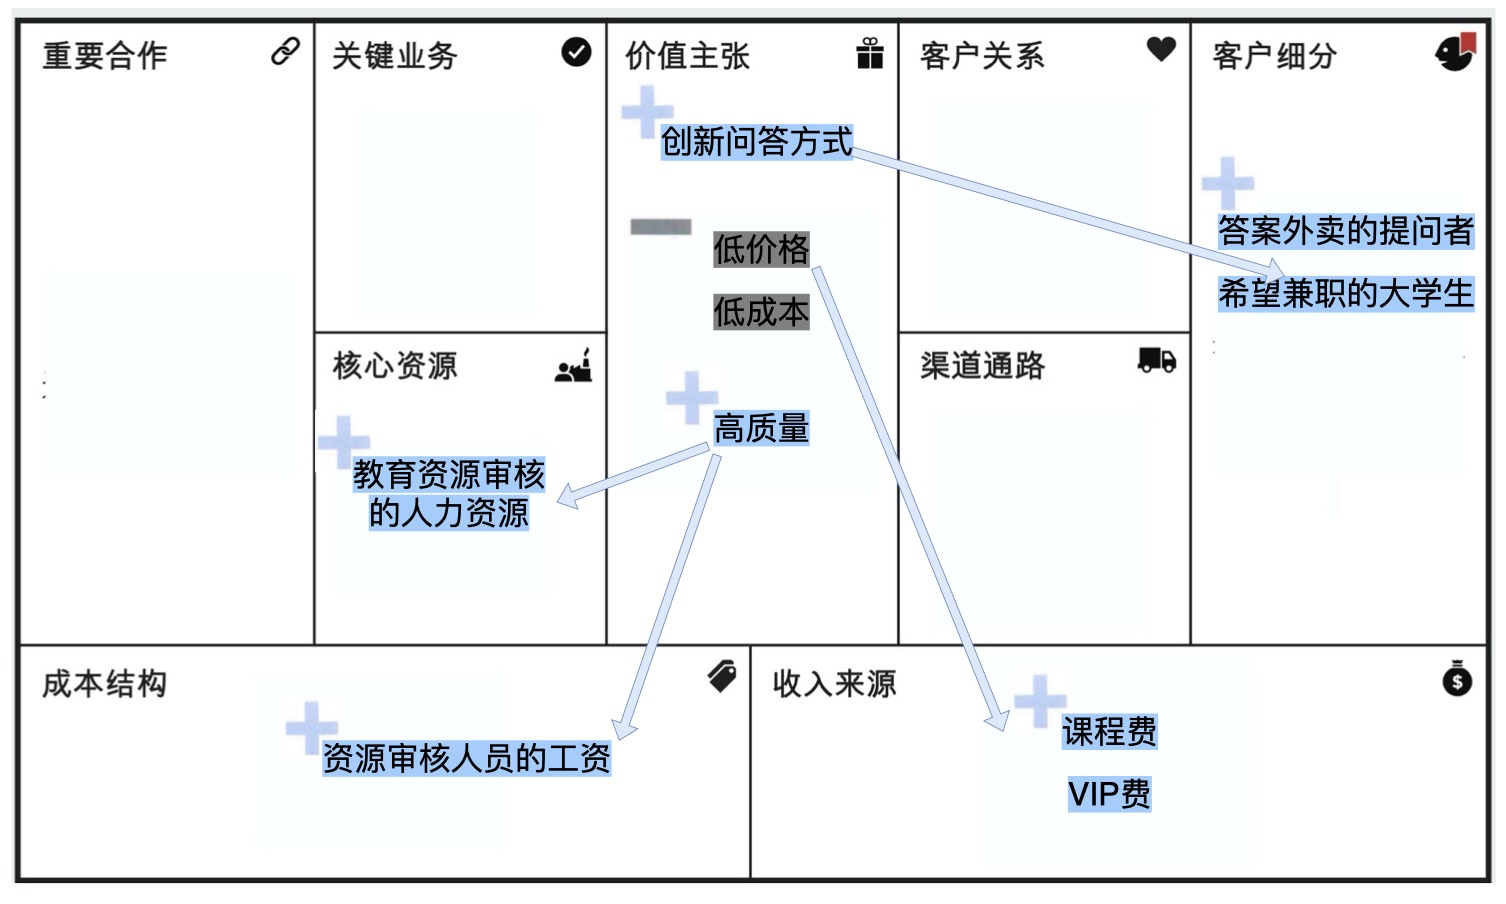
\includegraphics[scale=0.3]{价值主张.png}
\end{center}

\begin{itemize}
  \item \textbf{删除}:低成本
  \item \textbf{削减}:低价格
  \item \textbf{提升}:创新问答方式,课程费,VIP费
  \item \textbf{创造}:高质量,网课审核分级的人力资源,网课审核分级的人力资源成本
\end{itemize}

我们的平台聚焦于编程教学,所以教学质量无疑是用户考量的最重要的因素之一。只有高质量的学习资源才会为平台赢得更多的价值,确保用户都能学到正确有用的知识,增加用户体验。反之,如果没有我们没有太过于注重教学资源的“高质量”,会降低平台本身的价值,流失客户。所以为了确保学习资源的高质量,我们需要将网课进行审核分级,对“解答小哥”的技术水平进行考量,对问答平台的帖子的质量进行审核。

此外我们还要增强创新问答方式,这种方式主要基于平台特色的docker环境,其他类似平台还没有相似的功能,所以这对我们平台来说是很有竞争力的。通过这个业务我们可以收获更多的用户,比如我们的答案外卖提问者和兼职大学生等。让用户在学习过程中有前所未有的“答案外卖”的新体验。

当然这也会对核心资源和成本结构产生一些影响。平台增加了对教育资源审核分级的人力资源,同时为了支付这些人的工资,会增加一部分的成本。低成本和高质量这两个条件很难同时满足。比如我们要做到在承载大量用户的情况下,平台仍然可以流畅运行,我们必须要购进大量的先进的服务器,但是大量服务器必然会花费到更多成本;而且当聘请一些优质认证工程师和教师的时候,越优秀的工程师和教师所需要的合作费越多,在平台开展的初期,我们还需要花费许多宣传费用来帮助积累用户资源,提升平台的知名度,这些举动虽然会增加成本但是会保证平台的质量。我们应该优先考虑教育平台的质量,所以先删除低成本这一价值主张。

同时为了不让平台亏损,我们可以适当增加收入来源(即增加价格),将收费项目阶梯化,比如用户看某些普通网课视频的时候免费,看优质网课视频的时候收取少量费用,看名师网课视频的时候收取更多的费用。毕竟平台为了获取优质网课资源的同时也同样花费了大量成本。我们也可以打造阶梯化费会员(VIP会员,SVIP会员),VIP会员解锁部分权限(如:畅享部分网课,免去10次解答费),SVIP会员解锁全部权限(如:畅享全部网课,免去所有解答费用)。虽然提升价格可能会轻微打击用户使用平台的积极性,但是我们拥有其他平台没有的“答案外卖”的功能,而且网课、问答和文档资源都确保正确精致,用户足以被我们的高质量和创新所打动,可以抓住更多忠诚度高的用户。

\subsection{成本分析}
\begin{center}
  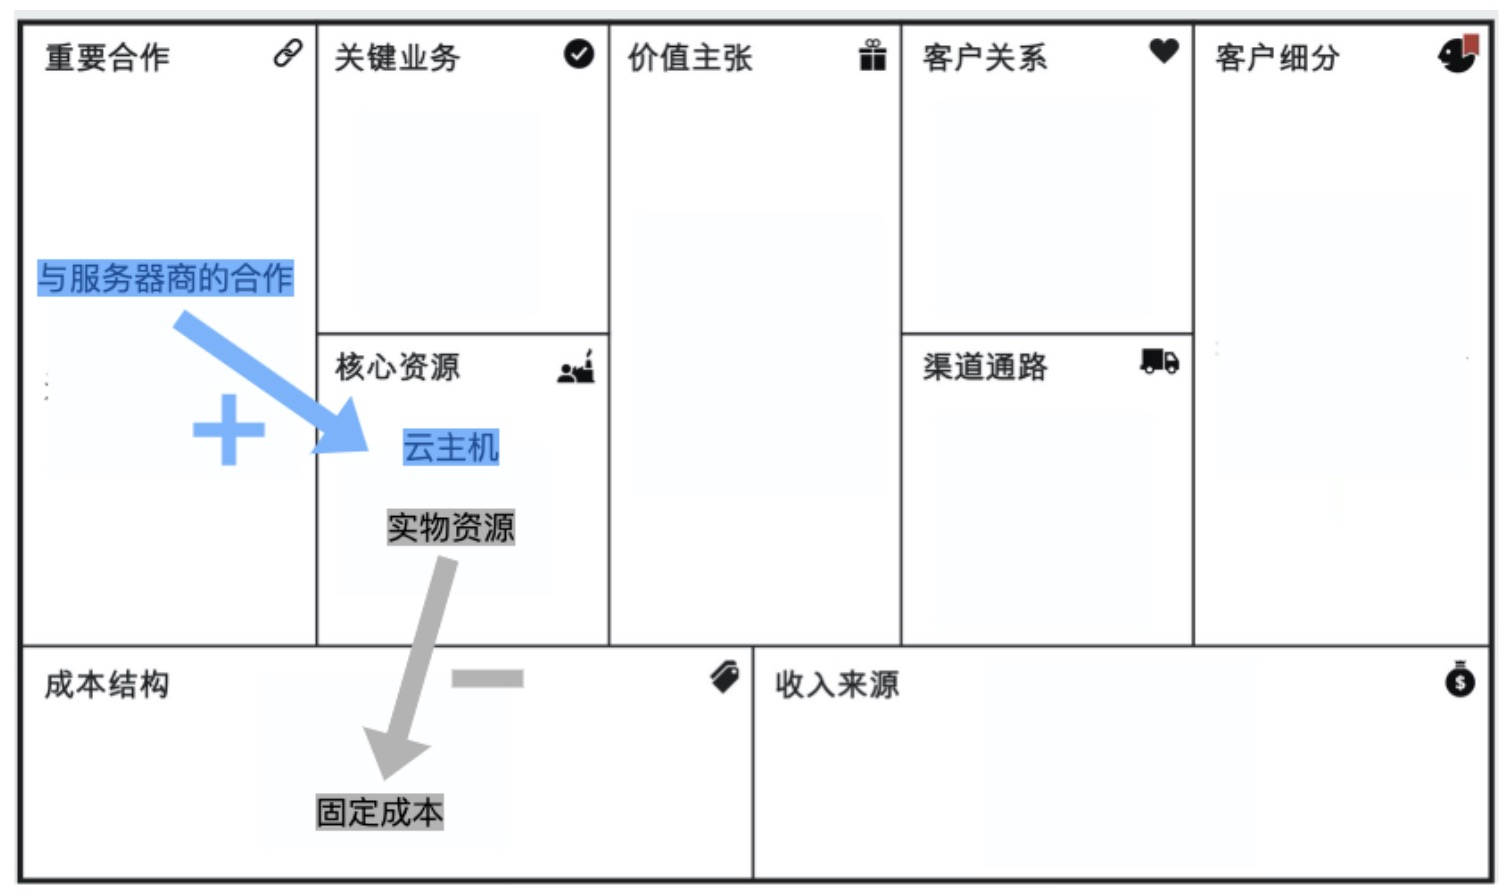
\includegraphics[scale=0.3]{成本分析.png}
\end{center}

\begin{itemize}
  \item \textbf{删除}:实物资源
  \item \textbf{削减}:固定成本
  \item \textbf{增加}:与服务器商的合作
  \item \textbf{创造}:云服务器
\end{itemize}

经过讨论,我们发现我们的初期成本过高,为此,我们应该利充分利用云计算资源:

首先,我们来关注核心资源部分,其中的实物资源主要是指我们自有的服务器等,经过综合考虑,我们认为不应再建立自有机房,为了保证全国各地用户的流畅访问,我们需要在多地部署机房,这不仅需要高昂的场地费、设备费、维护费,而且一旦发生故障,将造成一定数量的用户无法访问。我们的平台具有及时互动性,即使短时间的无法访问,也会对用户体验造成巨大影响。对于初期运营的我们来说,这样的费用与风险是难以承受的。

其次是成本部分,其中的固定成本主要来自于机房的场地费用、维护费用等,迁移至云端后,我们只需要按需支付云服务使用费,相比于固定成本,这样的好处主要是,我们不必再为准备资源的多少而精打细算。我们的平台具有时效性,例如,在寒暑假,来本平台学习的学生可能会更多,而在春秋季,则会进入淡季。按照原来的固定成本方案,如果我们购买的服务器过多,则会造成资源、金钱的浪费,而如果我们购置的资源过少,则会降低用户体验,造成客户流失,并且后续的扩容还需投入大量人力、精力。

在重要合作一项中,与服务器商的合作原本的优先级并不高,但是经过讨论,我们现在认为与服务器商的合作变得十分重要。我们需要在全国各地部署我们的服务,同时,为了保证服务的高可用性,我们需要同时将服务部署于多个云平台,如果能与服务器商取得一定的合作,降低云服务单价,那么将会减少我们相当大的成本。我们的平台自然也会有许多教大家搭建环境、部署服务的课程,我们可以在这种课程中介绍与我们有合作关系的服务器商,鼓励学员使用这些服务商的主机进行操作,为他们提供引流,增加其潜在用户量,从而为我们自身争取更大的优惠。

经过这番改造,云服务器也会成为我们的核心资源之一,尽管服务器本身并不归属于我们,但是相关的配置、组织、架构等等都是我们重要的资源。

\section{画布更新}

\subsection{整体描述}
整体来说,我们在画布的关键业务和核心资源上进行了一些调整。结合先前的分析,我们认为在编程课程的市场比之前的设想更大,因此深化了编程课程的业务,决定建立多级的课程分类来满足市场中不同类型客户的需要。同时利用现有资源增加面向企业的docker配置出租服务,在客户群体上的业务分配更加均衡,也可以增加收入。除此之外,跟进互联网发展趋势,利用云服务器平台,优化我们的服务器资源,以降低成本,也能更好地支持新增的docker配置出租业务。其余画布上的改变也都由这些改变引起,包括成本与价值主张等。

在关键业务上,网课教学会呈现多级的课程,以满足不同层次的用户的需求:时间不充裕的客户可以修习时长与负担都比较小的课程,能力较强的客户可以选择修习高级课程来精进能力等;docker配置出租意指向企业提供出租docker环境(可根据要求进行定制化配置和管理)的服务。多级课程的模型自然地改变了我们的价值主张,使用高性价比取代了低价格的课程定位——每位客户选择适合自己情况的课程来修习,课程的总体完成概率更高,客户的收获也个更多。收入上,docker配置出租服务会增加收入。

因为当下各种云服务器平台崛起,规模效应使云服务器的成本低于自行维护服务器的成本,应且还有易于配置,可伸缩等特性。从多方面考虑,确定我们的平台完全使用云服务器存储资源,开展服务,因此将服务器资源从实体资源中剥离出来,设立单独的云主机资源进行度量。进而与服务器厂商的合作关系的重要性相较之前大大地提升了。通过合作获得的价格优惠,会可观地影响云主机资源所产生的成本。另外我们也将其归类为可变成本,因为平台所租赁的云主机资源的规模可以随着平台不同的运行情况而发生改变,进而成本是不固定的。

最后我们发现我们的渠道通路比较薄弱,决定新增优惠制度,来鼓励我们的用户去邀请更多的人来使用我们的平台,以此补强我们的渠道通路。另外考虑到作用有限以及建设更优质干净的平台的需要,在评估过后,我们决定删除广告商这一客户群体,进而删除了广告费用的收入。

\subsection{画布更新可视化}
\begin{center}
  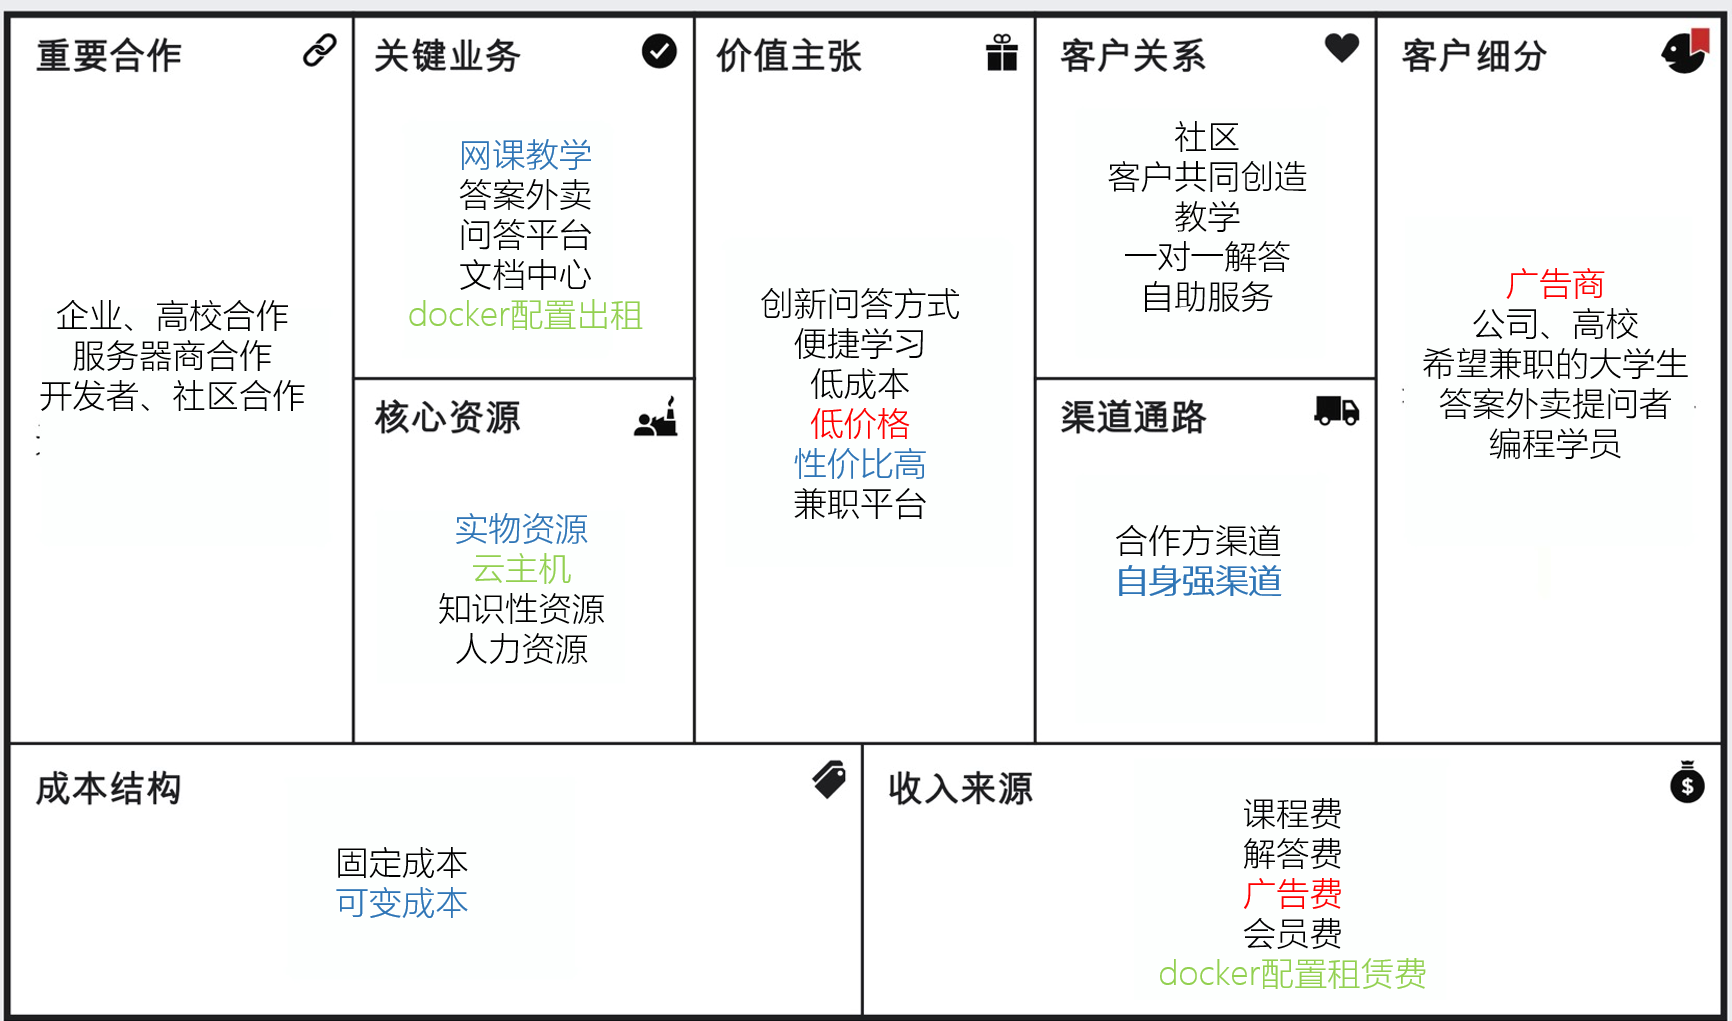
\includegraphics[scale=0.55]{更新后的画布.png}
\end{center}

绿色代表为新加项,蓝色代表修改项,红色代表删除项。

\subsection{商业画布详情}

最后,我们的商业模式画布如下

\begin{itemize}
  \item \textbf{关键业务}:平台主打业务为教育相关,具体分为网课教学和答案外卖两个核心,结合docker环境部署可运行的问答环境,降低用户的交流成本,尤其适用于计算机相关学科和问题的问答交流。细化这两项业务,我们提出了使用分级的课程来满足不同用户的不同需求。另外提供文档中心,相较于传统的文档,直接执行代码省去了用户配置环境、切换窗口、复制粘贴的时间,保障了用户思维的连续性,增加了用户学习 的效率。相较于博客,在文档中心,经典的算法、程序片段等同样的内容仅出现一次,并由用户不断完善,避免了用户在海量博文中进行寻找与甄别,节约了用户的时间。
  \item \textbf{价值主张}:平台为教育相关,因此价值主张围绕便捷学习、低成本、性价比和创新问答等展开。力求提供一个宽松、积极、互相交流、互帮互助的社区氛围。在计算机这个学科中,本身就崇尚开源精神,我们平台也将秉持这个理念,提供一个灵活、用户共同创造的问答和教育平台,以契合整个领域内的开源风气。另外,我们平台希望通过使用docker的问答环境能提供一种新的创新问答方式,激发问答双方更大的创造力。针对课程和付费问答业务,我们平台也可以作为一个兼职平台为用户提供第二份收入。
  \item \textbf{客户关系}:顺应我们的价值主张,主要维护社区、客户共同创造的氛围。另外,除了面向大众的问答,我们平台还致力于提供一个一对一问答的环境,让有着专业需求的用户可以和业界大拿一对一交流。灵活的客户关系有利于发挥各个回答者和教师的特长,也有助于客户发现最适合自己的服务。
  \item \textbf{客户细分}:我们的核心业务决定了平台主要的用户。一类是提出问题的提问者,这些提问者同时也是网课潜在的学生客户。这类客户是初入领域的编程学员,他们的需求主要是解决自己在编程中遇到的问题,或是学习编程方面的知识;而平台的另一类客户就是回答者和开设网课的教师群体,这类客户可以是自身的教授和工程师,也可以是希望兼职的优秀大学生,课余时间来解答其他学员提出的问题。这两大类客户群体大多来自于公司和高校,因此公司的工作人员和高校的教工和学生是我们潜在的客户群体。
  \item \textbf{渠道通路}:对应我们的客户群体,我们需要在公司和高校内部加强宣传,为了打通和公司和高校之间的联系,我们积极扩展我们的合作项目,同时加强熟人宣传,在高校和业界内形成良好的口碑,打造专业的品牌形象,以此来开拓渠道。同时,我们平台也提供人工客服等来提升用户使用体验和网课售后评价服务。
  \item \textbf{核心资源}:因为我们平台主要是线上平台,知识性资源仍然是我们的主要资源,包括网课资源和问答资源。这些问答的资料是我们用户留存和吸引流量的重要资源。同时,我们平台大量使用docker技术,因此对于云基础设施的需求和建设投入极大。docker的广泛使用有利于降低我们平台初期投入的成本,而云平台也是我们后期准备自研并且提供租赁服务的另一个核心资源。
  \item \textbf{成本结构}:我们的业务和资源决定了我们平台的成本有两类。首先是人力资源成本,这类成本大多是可变成本,主要是用于吸引优质教师和优秀回答者的成本,以及人工客服的成本等。另外一方面,我们平台需要有一定的基础设施来开展我们的平台建设,这一类固定成本主要来自于一些服务器的成本和开发人员的工资成本。
  \item \textbf{收入来源}:对应我们的核心业务,我们的收入来自于课程费、问答费和后期docker的租赁费用。另外,为了提高用户的留存率,我们还提出了会员制度。因此会员费也是我们的收入来源之一。
  \item \textbf{重要合作}:我们的渠道通路和客户细分决定了我们的重要合作。主要来自于企业、高校和开发者社区。他们都是我们潜在的客户来源。另外,我们还需要和服务器厂商合作,以此来降低我们初期的成本,并且为我们后期提供docker的租赁服务提供保障。
\end{itemize}



\end{document}